\documentclass[
  bibliography=totoc,     % Literatur im Inhaltsverzeichnis
  captions=tableheading,  % Tabellenüberschriften
  titlepage=firstiscover, % Titelseite ist Deckblatt
  parskip=half,
  ngerman
]{scrartcl}

% Paket float verbessern
\usepackage{scrhack}

% Warnung, falls nochmal kompiliert werden muss
\usepackage[aux]{rerunfilecheck}

% unverzichtbare Mathe-Befehle
\usepackage{amsmath}
% viele Mathe-Symbole
\usepackage{amssymb}
% Erweiterungen für amsmath
\usepackage{mathtools}

% Fonteinstellungen

% Latin Modern Fonts werden automatisch geladen
% Alternativ zum Beispiel:
%\setromanfont{Libertinus Serif}
%\setsansfont{Libertinus Sans}
%\setmonofont{Libertinus Mono}

% Wenn man andere Schriftarten gesetzt hat,
% sollte man das Seiten-Layout neu berechnen lassen
\recalctypearea{}

% deutsche Spracheinstellungen
\usepackage[main=ngerman]{babel}

%----------------
% Mathematik-Stil nach ISO
%----------------
\usepackage[
  math-style=ISO,
  bold-style=ISO,
  sans-style=italic,
  nabla=upright,
  partial=upright,
  warnings-off={
    mathtools-colon,
    mathtools-overbracket,
  },
]{unicode-math}

% traditionelle Fonts für Mathematik
\setmathfont{Latin Modern Math}
\setmathfont{XITS Math}[range={scr, bfscr}]
\setmathfont{XITS Math}[range={cal, bfcal}, StylisticSet=1]

% Zahlen und Einheiten
\usepackage[
  locale=DE,
  separate-uncertainty=true,
  per-mode=symbol-or-fraction,
]{siunitx}

% chemische Formeln
\usepackage[
  version=4,
  math-greek=default,
  text-greek=default,
]{mhchem}

% richtige Anführungszeichen
\usepackage[autostyle]{csquotes}

% schöne Brüche im Text
\usepackage{xfrac}

% Standardplatzierung für Floats einstellen
\usepackage{float}
\floatplacement{figure}{htbp}
\floatplacement{table}{htbp}

% Floats innerhalb einer Section halten
\usepackage[
  section,
]{placeins}
\makeatletter
\AtBeginDocument{%
  \expandafter\renewcommand\expandafter\subsection\expandafter{%
    \expandafter\@fb@secFB\subsection
  }%
}
\makeatother

% Seite drehen für breite Tabellen: landscape Umgebung
\usepackage{pdflscape}

% Seitenränder temporär kleiner machen
\usepackage{geometry}

% Captions schöner machen.
\usepackage[
  labelfont=bf,
  font=small,
  width=0.9\textwidth,
]{caption}
% subfigure, subtable, subref
\usepackage{subcaption}

% Grafiken können eingebunden werden
\usepackage{graphicx}
\usepackage{grffile}
\graphicspath{{./bilder/}{./}}


% schöne Tabellen
\usepackage{booktabs}

% Verbesserungen am Schriftbild
\usepackage{microtype}

% Literaturverzeichnis
%\usepackage[
 % backend=biber,
 % natbib=true,
 % style=numeric,
 % sorting=none
%]{biblatex}
%\addbibresource{../bib/lit.bib}
%\addbibresource{../bib/programme.bib}
%\addbibresource{../bib/versuche.bib}

% Hyperlinks im Dokument
\usepackage[
  german,
  unicode,
  pdfusetitle,
  pdfcreator={},
  pdfproducer={},
]{hyperref}
\usepackage{hyperref}

% erweiterte Bookmarks im PDF
\usepackage{bookmark}

% Trennung von Wörtern mit Strichen
\usepackage[shortcuts]{extdash}

% Anpassbare Enumerates/Itemizes
\usepackage{enumitem}

% Tabellen mit einer Zelle über mehrere Reihen
\usepackage{multirow}

% Tabellen aus .csv Dateien
\usepackage{csvsimple}

%----------------
% Neue Commands
%----------------
\NewDocumentCommand \dif{m}{
  \mathinner{\symup{d} #1}
}
\NewDocumentCommand \tableSI{m m}{
  $#1 \:/\: \si{#2}$
}

%----------------
% Autoreninformationen
%----------------

\author{%
  Jannes Krause\\
  \href{mailto:jannes.krause@tu-dortmund.de}{jannes.krause@tu-dortmund.de}%
  \and
  Lea Krüger\\
  \href{mailto:lea.krueger@tu-dortmund.de}{lea.krueger@tu-dortmund.de}%
}





 

\begin{document}

\subject{V60}
\title{Der Diodenlaser} \date{Durchführung: 11.11.2026 \\ Abgabe: 25.11.2026 }

\maketitle
\thispagestyle{empty}

\clearpage

\pagenumbering{Roman}
\tableofcontents
\clearpage

\pagenumbering{arabic}

\section{Zielsetzung}

Der vorliegende Versuch hat den Diodenlaser zum Thema, welcher als Halbleiterlaser Licht durch stimulierte Emission innerhalb einer Halbleiterstruktur erzeugt.
Allgemein zeichnet sich Laserlicht durch eine hohe Lichtintensität bei eng begrenzter Frequenzbandbreite, hoher Kohärenz und gleicher Polarisation aus, was 
es neben vielen anderen Anwendungen bestens zur Untersuchung optischer atomarer Übergänge qualifiziert.
Einige Eigenschaften des im Diodenlaser erzeugten Laserlichtes, sowie die Möglichkeiten zu dessen Manipulation werden nun im nachfolgend besprochenen Versuchsaufbau 
sichtbar gemacht. Als exemplarische physikalische Anwendung wird mit dessen Hilfe das Transmissionsspektrum von Rubidiumdampf aufgenommen.






\section{Theorie}

\subsection{Relevante Grundlagen aus der Halbleiterphysik}

\subsubsection{Valenz- und Leitungsband in Halbleitern und Dotierung}

Für ein grundlegendes Verständnis der Funktionsweise und der Eigenschaften des Diodenlasers muss die Physik der Halbleiter und deren elektronische
Bandstruktur betrachtet werden.
Im Kontrast zu elektrischen Leitern existieren in reinen Halbleitern im Grundzustand kaum freie Ladungsträger zum eletrischen Stromstransport.
Valenz- und Leitungsband sind jedoch durch eine im Vergleich zu Isolatoren kleine Bandlücke voneinander getrennt, sodass bereits eine geringe Energiezufuhr in Form von Wärme, Licht oder elektrischer Spannung zur einer Erhöhung 
der elektrischen Leitfähigkeit dieser Materialien führt.\cite{grundwissenHalbleiter}
Diese Tasache liegt bei der Lokalisation der Fermienergie des Halbleiters begründet, also die maximale Elektronenenergie im Material am absoluten Nullpunkt, die hier zwischen Valenz- und Leitungsband liegt.
\autoref{fig:bandstruktur} stellt die Bandstrukturen von Leitern, Halbleitern und Isolatoren schematisch dar.

\begin{figure}[H]
    \centering
    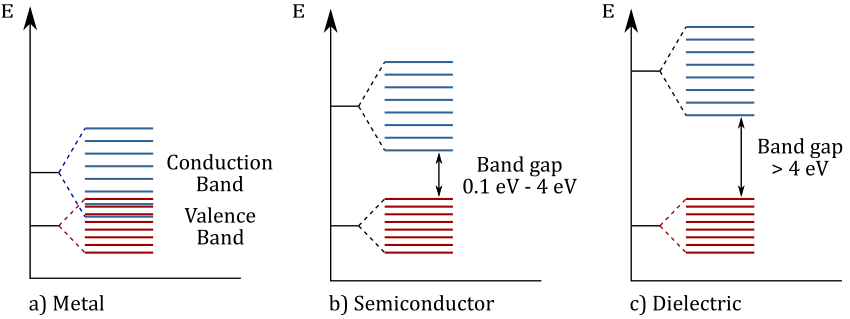
\includegraphics[width=0.8\textwidth]{bilder/band-structure.png}
    \caption{Schematische Bandstruktur eines Leiters, Halbleiters und Dielektrikums \cite{suetterlin2020}.}
    \label{fig:bandstruktur}
\end{figure}

Die Dotierung bezeichnet die Gesamtheit aller Verfahren, mit deren Hilfe bestimmte Fremdatome in den Halbleiter eingebracht werden, um gezielt dessen elektrische Leitfähigkeit
zu beeinflussen. So werden bei der p-Dotierung Fremdatome eines Elementes mit einer im Vergleich geringeren Anzahl von Valenzelektronen, typischerweise also Elemente
niedrigerer Hauptgruppennummer, in den Halbleiter eingebracht. Es entstehen ein sogennantes "Loch", die sich bei Anlegen einer Spannung wie positive Ladungsträger verhalten.
Energetisch liegt dieses knapp oberhalb des Valenzbandes, sodass durch geringe Anregung eine raumfeste negative Ladung im Gitter, sowie eine bewegliche Elektronenfehlstelle entsteht.
Im umgekerten Fall werden bei der n-Dotierung Elemente mit vergleichsweise größerer Zahl von Valenzelektronen in den Halbleiter eingebracht, hier werden die Ladungsträger
schlicht als Elektronen bezeichnet. Diese liegen knapp unterhalb des Leitungsbandes und können durch geringe Energiezufuhr ins Leitungsband überführt werden, wo sie 
für den elektrischen Stromtransport zur verfügung stehen. Dementsprechend entsteht eine ortsfeste positive Ladung im Kristallgitter.

\subsubsection{pn- Übergang und Dioden}

Beim Zusammenbringen unterschiedlich dotierter Halbleiter kommt es zu einer Wanderung von Elektronen aus der n-dotierten in die p-dotierte Schicht und umgekehrt zur
Migration von Löchern in die n-dotierte Schicht.
In diesem als pn- Übergang bezeichneten Bereich entsteht eine Raumladungszone mit einem elektrischen Feld, welches nun eine polungsabhängige Durchlass- oder Sperrrichtung bei Anlegen einer Spannung
konstituiert. In \autoref{fig:pn-uebergang} ist dieser Vorgang skizziert dargestellt.
Ein so konstruiertes elektronisches Bauteil wird als Diode bezeichnet und bildet die Grundlage für den Diodenlaser. Bei Anlegen einer Spannung in Durchlassrichtung wird das 
elektrische Feld in dem auch als Verarmungszone bezeichneten Raumladungszone abgebaut und elektrischer Strom fließt unter Rekombination von Elektronen aus dem Leitungs- und Löchern
aus dem Valenzband. Die Energiedifferenz wird hierbei in Form eines Photons frei. 


\begin{figure}[H]
    \centering
    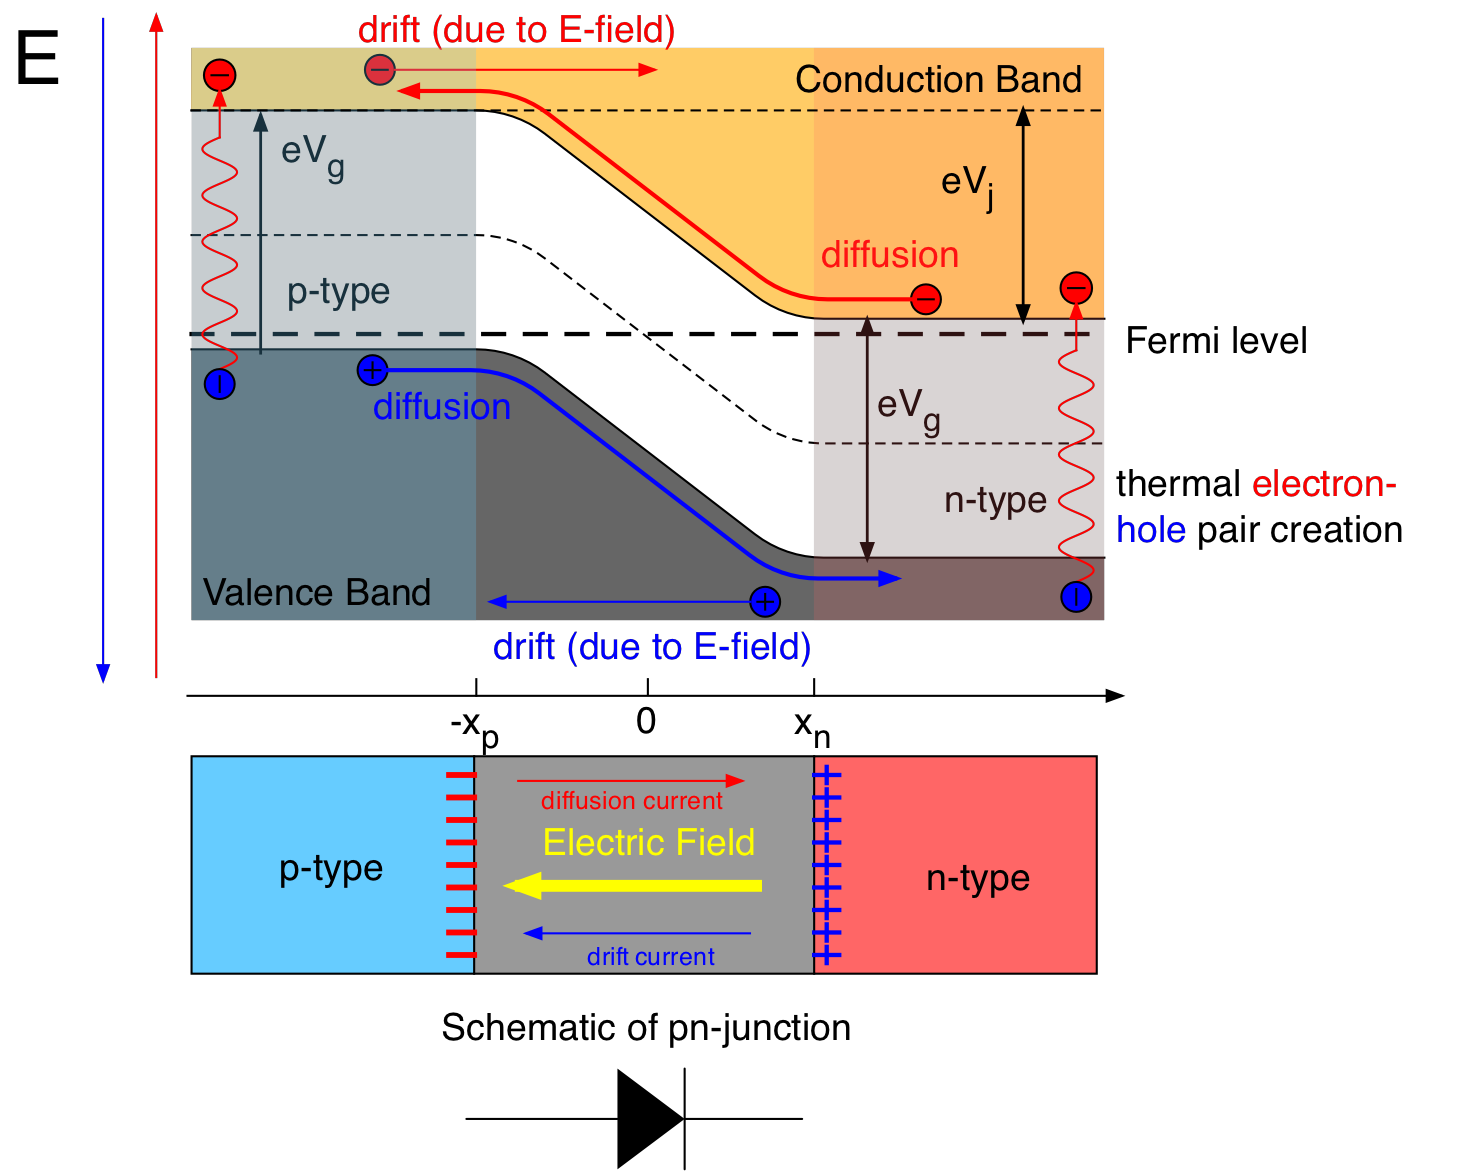
\includegraphics[width=0.8\textwidth]{bilder/pn-junction_energy.png}
    \caption{Schematische Darstellung eines p-n-Übergangs \cite{boeglinPNJunction}.}
    \label{fig:pn-uebergang}
\end{figure}




\subsection{Grundlagen aus Optik und Laserphysik}

\subsubsection{Kohärenz}

Zum Verständnis des Phänomens der Kohärenz wird Licht als die räumliche und zeitliche Ausbreitung elektromagnetischer Wellen betrachtet.
Bei Überlagerung verschiedener elektromagnetsicher Felder kann bei einer festen Phasenbeziehung ebendieser Interferenz beobachtet werden, eine räumlich stationäre
Feldamplitude der Überlagerung.\cite{kohaerenz}
Die Kohärenzzeit $\tau_{\mathrm{c}}$ gibt die zeitliche Dauer dieser festen Phasenbeziehung an und steht mit der spektralen Breite $\Delta \nu$
in der Bezehung

\begin{equation*}
\tau_{\mathrm{c}} = \frac{1}{\Delta \nu}.
\end{equation*}

Diese Reziprozität zeigt, dass für kohärentes Licht eine möglich enge Frequenzbandbreite des Lichtes erforderlich ist.
Es lässt sich mit der Vakuumlichtgeschwindigkeit $c$ auch eine Kohärenzlänge

\begin{equation*}
l_{\mathrm{c}} = c\,\tau_{\mathrm{c}}
\end{equation*}

definieren, die die Strecke dieser festen Phasenbeziehung angibt.
Als \textit{Kohärenz 1. Ordnung}

\begin{equation*}
g^{(1)}(\tau)
=
\frac{\left\langle E^*(t)\,E(t+\tau)\right\rangle}
{\left\langle E^*(t)\,E(t)\right\rangle}
\end{equation*}

wird die Korrelation des elektromagnetischen Feldes zu den Zeitpunkten $t$ und $t+\tau$ verstanden. $g^{(1)}(\tau)$ nimmt Werte zwischen $0$ und $1$ an, wobei
bei $1$ vollständige und bei $0$ keine Kohärenz des elektromagnetischen Feldes vorliegt.(Vgl. \cite{steck_coherence})
Allgemein zeichnet sich Laserlicht durch eine hohe Kohärenz 1. Ordnung aus, während das Licht von Glühlampen aufgrund der thermischen Entstehung der Strahlung
eine weitaus geringere Kohärenz aufweist.
Die \textit{Kohärenz 2. Ordnung} 

\begin{equation*}
g^{(2)}(\tau)
=
\frac{\left\langle I(t)\,I(t+\tau)\right\rangle}
{\left\langle I(t)\right\rangle^2}
\end{equation*}


betrachtet demgegenüber die Korrelation der Intensität $I$ zu verschiedenen Zeitpunkten, also, ob die Photonen des Lichtes gehäuft oder einzeln in einem Raumpunkt auftreffen.
Hier weist monochromatisches Licht als ideales Laserlicht einen Wert von $1$ auf, während weniger kohärentes Licht größerere Werte besitzt.(Vgl. \cite{steck_coherence})






\subsubsection{Photonen im Halbleiter, Laserlicht durch stimulierte Emission und Bestzungsinversion}

Für die Erzeugung von Laserlicht in einer Laserdiode müssen drei Wechselwirkungen von Photonen und Elektronen im Halbleiter betrachtet werden.
Bei der \textit{spontanen Emission} kommt es zur selbstständigen Rekombination eines Elektron-Loch-Paares  und damit Aussendung eines Photons, dessen
Energie näherungsweise der Bandlücke entspricht. Dabei ist die Richtung der Emission, die Polaristation und Phase statistisch verteilt.
Umgekehrt kann ein Photon ebenso von einem Elektron im Valenzband aufgenommen und damit ein Elektron-Loch-Paar erzeugt werden, was als \textit{Absoption} bezeichnet wird.
Beide Prozesse finden mit derselben Wahrscheinlichkeit im Halbleiter statt.
Der für die Erzeugung des Laserlichtes verantwortliche Prozess ist die \textit{stimulierte Emission}, bei der ein einfallendes Photon ein Elektron-Loch-Paar
zur Rekombination und zum Aussenden eines Photons identischer Richtung, Phase und Polarisation führt. So kommt es durch positive Rückkopplung zu einem
starken Intensitätsanstieg kohärenten Lichtes, was als Laserlicht bezeichnet wird
In \autoref{fig:em_ab_stim} sind diese Prozesse gegenübergestellt.

\begin{figure}[H]
    \centering
    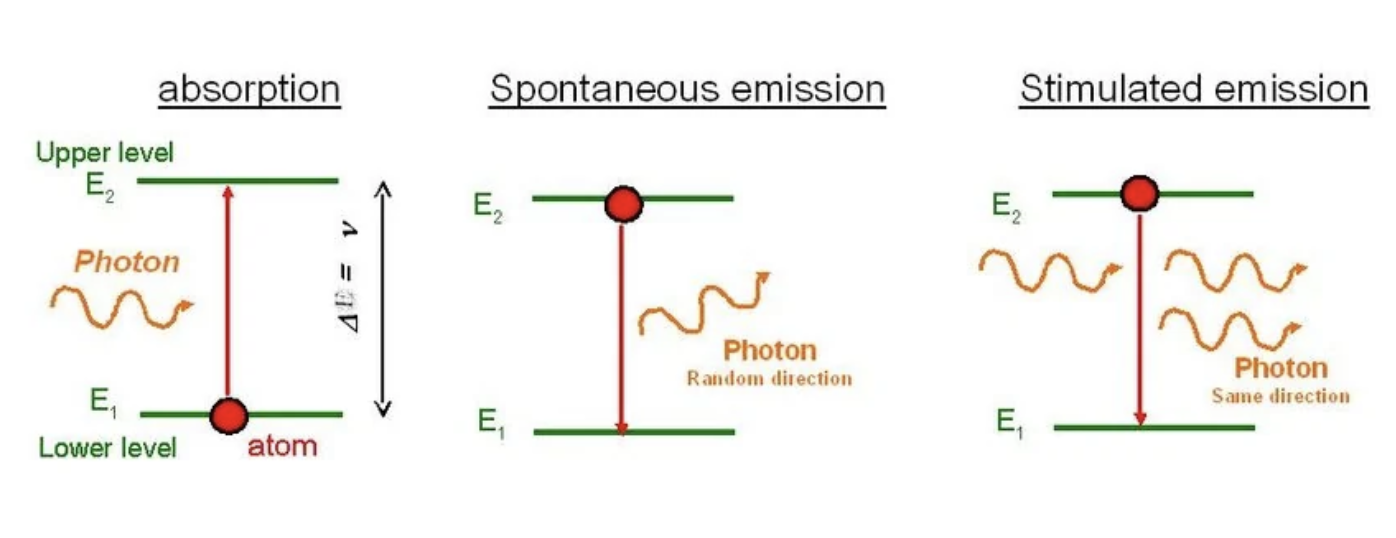
\includegraphics[width=0.8\textwidth]{bilder/em_ab_stim.png}
    \caption{Spontane Emission, Absorption und stimulierte Emission im halbleiter\cite{deMatos_absorption}.}
    \label{fig:em_ab_stim}
\end{figure}

Im thermischen Gleichgewicht übersteigt die Anzahl der Elektronen in niedrigeren die der Elektronen in angeregten Zuständen, hierdurch überwiegt der Prozess der Absorption
dem der stimulierten Emission. Ein Verschieben des Gleichgewichtes zu angregten Zuständen lässt sich mithilfe von Energiezufuhr,
im Falle des Diodenlasers Anlegen eines Pumpstromes, durch den Elektronen und Löcher in den Halbleiter injiziert werden, erreichen.
Allerdings muss für die Dominanz der stimulierten Emission ebenfalls ein Zustand der \textit{Besetzungsinversion} vorliegen:
Hiermit ist ein Überwiegen angeregter Elektronen gegenüber ebendieser im Grundzustand gemeint, welche in einem simplen Zweiniveausystem wie bisher präsentiert nicht erreicht 
werden kann. Sei hierzu angenommen, dass ein angeregter Energiezustand $E_2 > E_1$ höher besetzt sei. Aufgrund gleicher Wahrscheinlichkeit von spontaner Emissiom
und Absorption würde erstere alsbald zu einer Rückkehr zum Gleichgewicht zwischen beiden Niveaus führen, was eine gewünschte kaskadenartigen Zunahme der stimulierten
Emission im Halbleiter unmöglich macht. Erst und mindestens ein Dreiniveausystem macht eine dauerhafte Bestzungsinversion realisierbar.
Hier existiert ein weiteres angregtes Niveau $E_3$ oberhalb des für die stimulierte Emission zur Verfügung stehenden Energieniveaus $E_2$, in welches aus dem Grundzustand $E_1$
durch den Pumpstrom angeregt wird und aus dem Elektronen zügig strahlungslos in das als metastabil bezeichnete Niveau $E_2$ relaxieren. Ausreichende Pumpströme, 
bezeichnet als Schwellenstrom $I_{\mathrm{th}}$, können so zu einer Besetzungsinversion mit Besetzungszahlen $N_2 > N_1$ zwischen den Energieniveaus $E_2$ und $E_1$ führen.
In einem Vierniveausystem liegt hingegen stets Bestzungsinversion mit $N_1 > N_2$ vor, hier existiert unterhalb des Niveaus $E_1$ noch ein weiteres Niveau $E_0$, aus 
dem in das Niveau $E_4$ gepumpt wird.\cite{mitofsky_laser}
In \autoref{fig:popinv} sind die beschriebenen Niveausysteme graphisch veranschaulicht.

\begin{figure}[H]
    \centering
    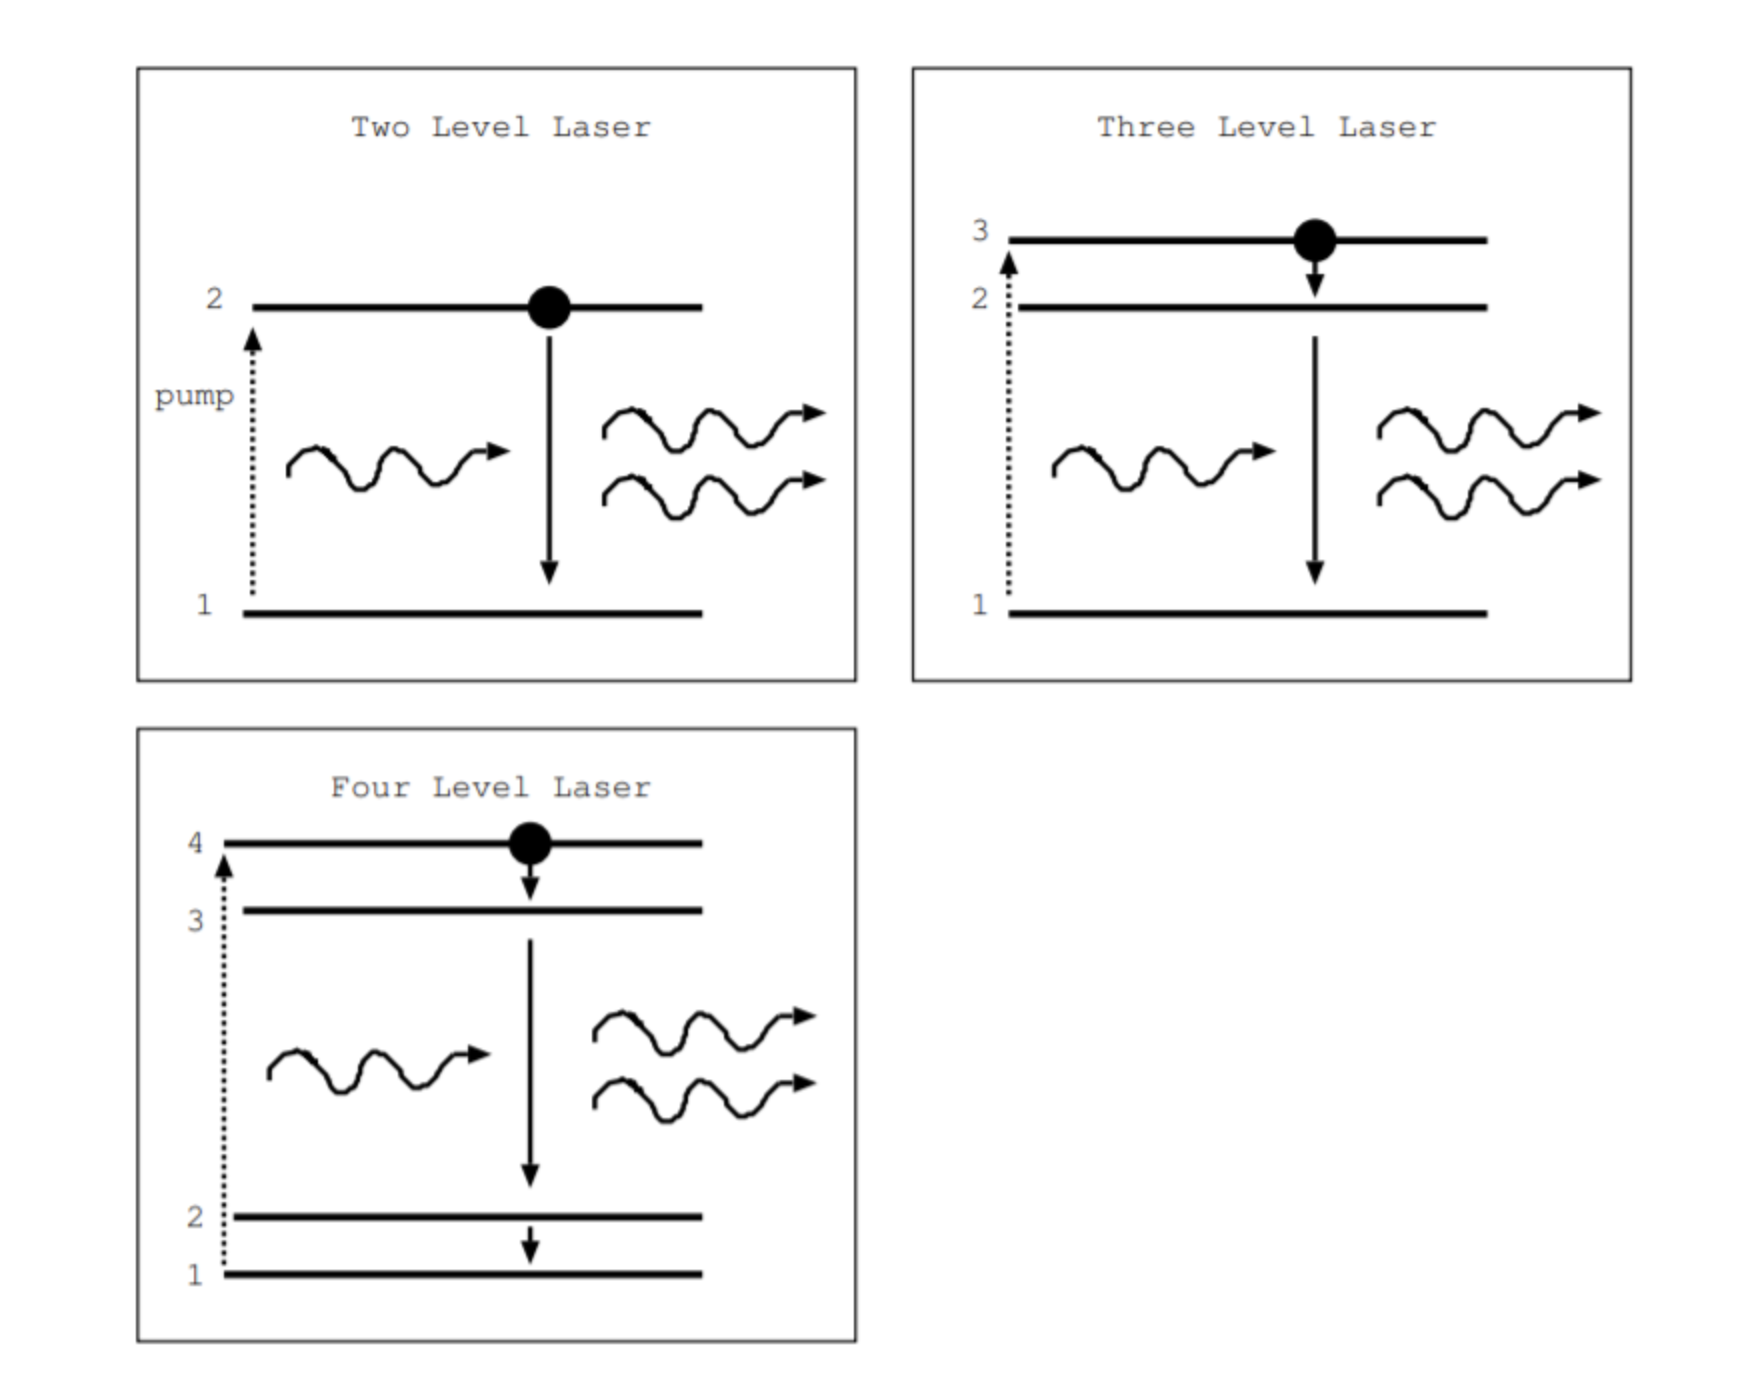
\includegraphics[width=0.8\textwidth]{bilder/popinv.png}
    \caption{Vergleich verschiedener Niveausysteme im Halbleiter\cite{mitofsky_laser}.}
    \label{fig:popinv}
\end{figure}















\subsection{Der Diodenlaser}

\subsubsection{Aufbau und allgemeine Funktionsweise des Diodenlasers}

Als Laserdiode werden entsprechende Halleiterchips verwendet, deren Konstruktion schematisch in \autoref{fig:hl-chip} zu sehen ist.
Über die Elektroden findet die Injektion der Ladungsträger in die Diode statt. Die p- und n-dotierte Halbleiterschichten sind hier als "cladding layers" bezeichnet. Der pn- Übergang, als "active layer" bezeichnet,
ist der Ort, an dem die Rekombination der Ladungsträger im Halbleiter und damit auch die spontane und stimulierte Emission stattfinden. Diese Schicht dient ebenfalls 
als optischer Wellenleiter, da sie einen höheren Brechungsindex als ihre Umgebung ausweist und so zu einem größeren Teil vollständig reflektiert wird.\cite{diodelaserphysics}
An einem langen Ende des Chips ist eine halbdurchlässige, am anderen eine vollreflektierende Schicht aufgetragen, deren Zwischenraum als interner Resonator bezeichnet wird
und das Erzeugen stehender elektromagnetischer Wellen im Chip ermöglicht. \autoref{fig:strahlung} zeigt die so entstehenden longitudinalen und transversalen Lasermoden.
Beim wiederkehrenden Durchgang durch die aktive Schicht vergrößert sich die Intensität des Laserlichtes, bis es schließlich an der halbdurchlässigen Seite des Chips austritt.
Die gesamte Diode sitzt auf einem Heat-Sink, über das die Temperatur der Diode eingestellt werden kann.
Zu kleine Pumpströme kompensieren die optischen Verluste innerhalb der aktiven Zone zu groß, sodass die Laserschwelle nicht erreicht und die Laserdiode im LED-Modus betrieben
wird. Dieser zeichnet sich gemäß seines Entstehungsvorgangs durch spontane Emission im Vergleich zum Laserlicht durch wesentlich geringere Intensität des Lichtes mit
geringerer Kohärenz und relativ große spektrale Breite aus.
Bei Erreichen des Schwellenstroms dominiert die stimulierte Emission als primärer lichterzeugender Vorgang, Ergebnis ist ein kohärenter Laserstrahl, dessen
Intensität nun linear mit dem Laserdiodenstrom ansteigt.\cite{diodelaserphysics}
Der primäre, aus der Diode austretende Laserstrahl ist zunächst divergent und in transversaler Richtung elliptisch geformt. Die Wellenlänge $\lambda$ des Laserlichtes entspricht ungefähr
der Bandlücke des verwendeten Halbleitermaterials.


\begin{figure}[H]
    \centering
    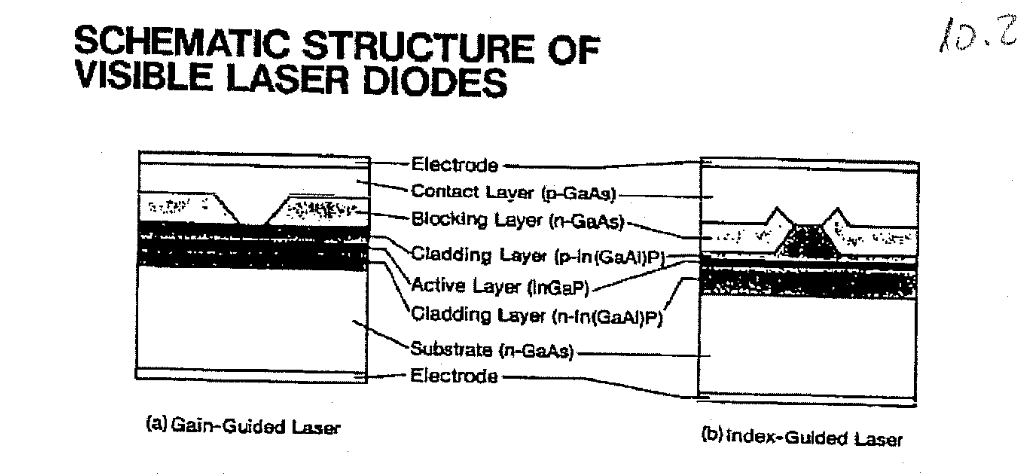
\includegraphics[width=0.8\textwidth]{bilder/hl-chip.png}
    \caption{Schematischer Aufbau einer Laserdiode \cite{diodelaserphysics}.}
    \label{fig:hl-chip}
\end{figure}



\begin{figure}[H]
    \centering
    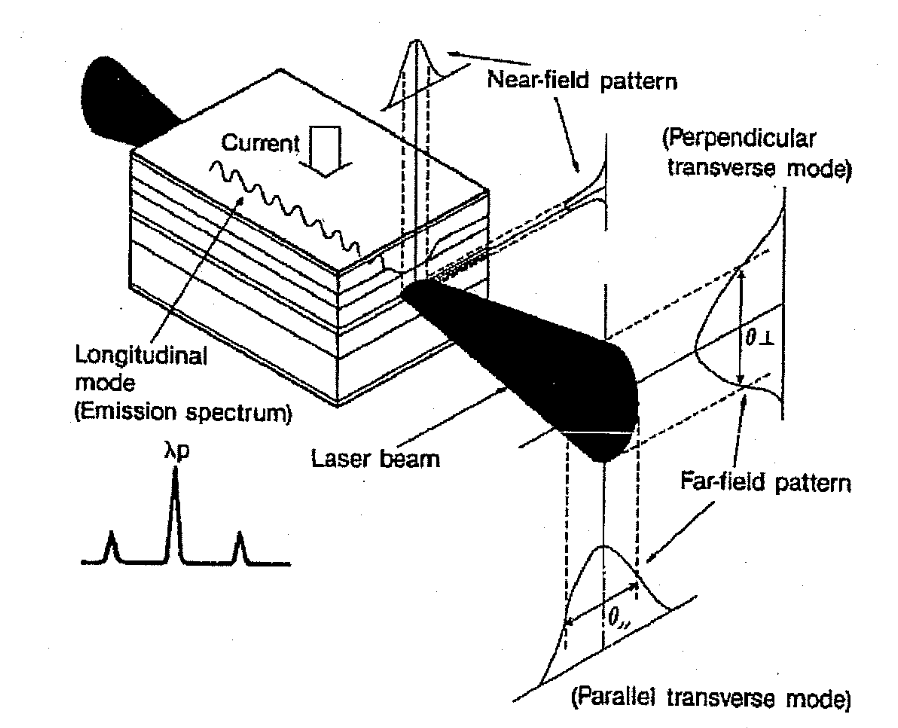
\includegraphics[width=0.8\textwidth]{bilder/strahlung.png}
    \caption{Longitudinale und transversale Lasermoden im Laserdioden-Halbleiterchip \cite{diodelaserphysics}.}
    \label{fig:strahlung}
\end{figure}


\subsubsection{Der Littrow-Aufbau}

Der gemäß bisheriger Beschreibung aufgebaute und betriebene Laser besitzt zunächst eine für Untersuchungen von atomaren Übergängen ungünstig große
Bandbreite von $\Delta \nu \approx 50\,\si{\mega\hertz}$.\cite{diodelaserphysics}
Der "Littrow-Aufbau", gezeigt in \autoref{fig:littrow}, erweitert den inneren Resonator des Diodenlasers um einen Kollimator zur Erzeugung einer annähernd planaren Wellenfront und ein außerhalb des Chips liegendes Beugungsgitter, welches eine kontrollierte
Rückkopplung in die aktive Schicht und damit eine Stabilisierung und Begrenzung der Bandbreite bis zu $\Delta \nu \approx 1\,\si{\mega\hertz}$
ermöglicht.\cite{diodelaserphysics}

\begin{figure}[H]
    \centering
    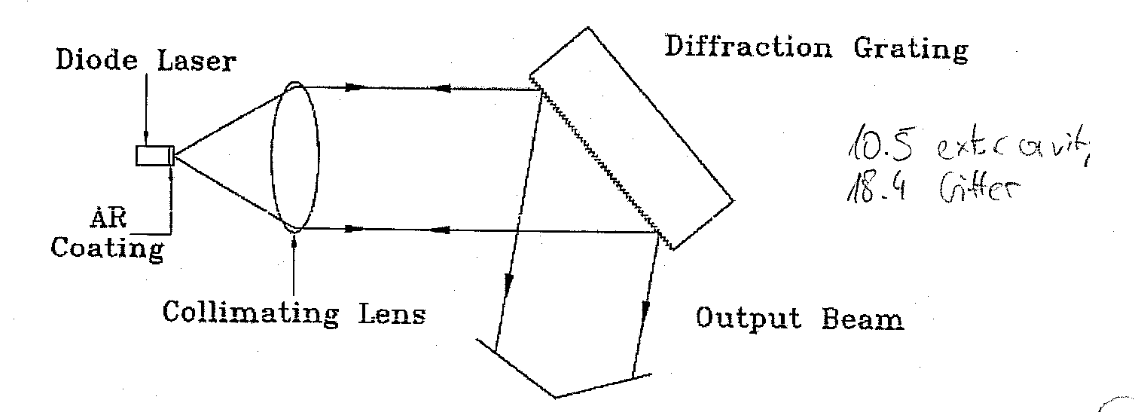
\includegraphics[width=0.8\textwidth]{bilder/littrow.png}
    \caption{Schema des Littrow-Aufbaus \cite{diodelaserphysics}.}
    \label{fig:littrow}
\end{figure}



Für die Wellenlänge $\lambda$  gilt die Gittergleichung

\begin{equation*}
    m \lambda = 2d \sin(\theta),
\end{equation*}

wobei $\theta$ dem Winkel zwischen einfallendem Laserstrahl und Normalen des Gitters bezeichnet und $m$ die Beugungsordnung darstellt, zumeist mit $m=1$.

\subsubsection{Auswahl von Lasermoden und Faktoren bei der Netto-Verstärkung}

Die Konstruktionsweise des Diodenlasers unter Miteinbeziehung des Littrow-Aufbaus gibt 4 Faktoren zur Einflussnahme auf die Frequenz und die Begrenzung der
Lasermoden auf die im vorliegenden Versuch erwünschte Einzelmodenemission zu, indem innerhalb der gesamten Bandbreite einzelne Wellenlängenbereiche verstärkt werden.
So strahlt der Diodenlaser bei der Frequenz mit der größten Netto-Verstärkung.\cite{diodelaserphysics}
Die Faktoren zur Einstellmöglichkeit sind:

\begin{enumerate}
    \item \textbf{Verstärkung im aktiven Medium}

    Die Größe der Bandlücke, abhängig vom verwendeten Halbleitermaterial und der Temperatur des Lasers erzeugen einen breiten Peak im Frequenzraum.
    \autoref{fig:verstaerk_aktmed} zeigt diese Abhängigkeiten, wobei die Temperatur des Lasers direkt durch den Pumpstrom beeinflusst wird.



    \begin{figure}[H]
        \centering
        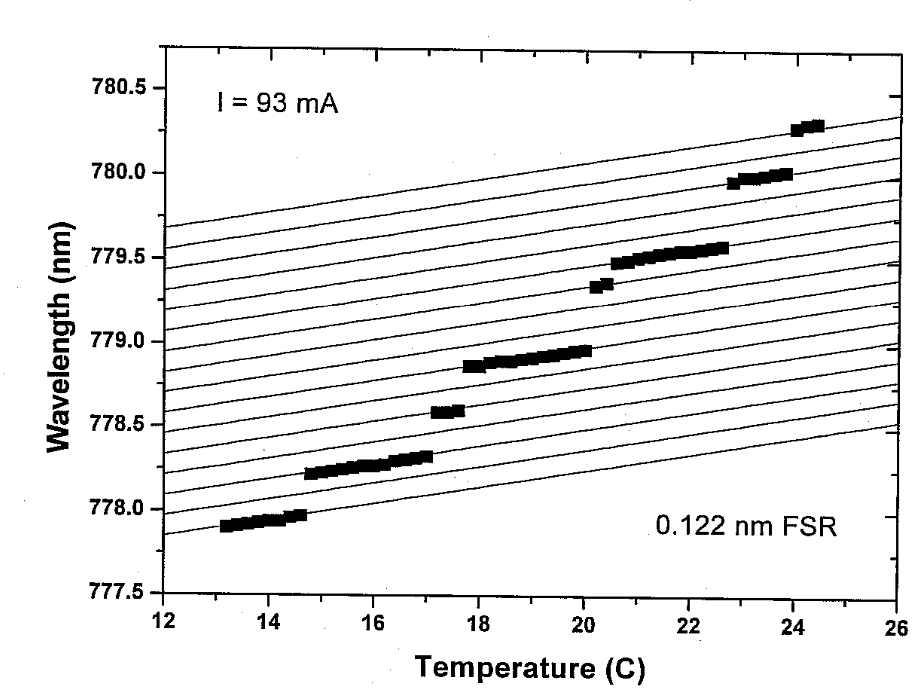
\includegraphics[width=0.7\textwidth]{bilder/verstaerk_aktmed.png}
        \caption{Die Wellenlänge des im aktiven Medium freigesetzten Laserlichts in Abhängigkeit von Temperatur und Pumpstrom.\cite{diodelaserphysics}}
        \label{fig:verstaerk_aktmed}
    \end{figure}

    \item \textbf{Verstärkung im internen Resonator}

    Die Länge $L$ des internen Resonators und der Brechnungsindex der aktiven Schicht $n$ konstituieren eine frequenzperiodische Verstärkung.
    Der Frequenzabstand der benachbarten longitudinalen Resonatormoden wird als "Freier Spektralbereich" bezeichnet und ergibt sich gemäß

    \begin{equation*}
        \Delta \nu_{\mathrm{FSR}} = \frac{c}{2nL}.
    \label{eq:FSR}
    \end{equation*}

    Die Frequenzverstärkungsfunktion des internen Resonators verschiebt sich abhängig von der Temperatur und dem Pumpstrom, die Temperaturabhängigkeit ergibt sich
    aus einer Größenänderung der Bandlücke, während der Pumpstrom einerseits die Temperatur beeinflusst, als auch den Brechungsindex der aktiven Schicht und damit
    ihre optische Länge verändert.\cite{diodelaserphysics}
    In \autoref{fig:verstaerk_intcav} ist die Abhängigkeit der im internen Resonator stehenden Wellenlänge vom Pumpstrom grafisch aufgetragen.

    \begin{figure}[H]
        \centering
        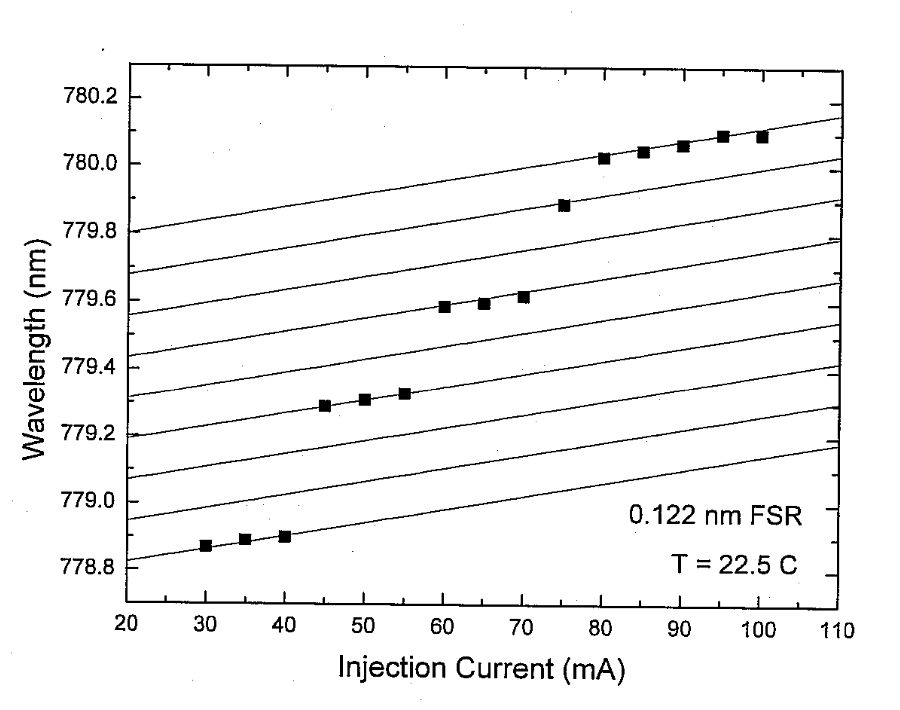
\includegraphics[width=0.7\textwidth]{bilder/verstaerk_intcav.png}
        \caption{Die Wellenlänge im internen Resonator in Abhängigkeit vom Pumpstrom.\cite{diodelaserphysics}}
        \label{fig:verstaerk_intcav}
    \end{figure}



    \item \textbf{Verstärkung durch Gitterrückkopplung}

    Durch die Beugung am Littrow-Gitter wird nur ein eng begrenzter Wellenlängenbereich in den Resonator rückgekoppelt und im Laser verstärkt.
    Die spektrale Breite der Beugung 1. Ordnung am Gitter $\Delta \nu$ ist gegeben durch 

    \begin{equation*}
        N = \frac{\nu}{\Delta \nu},
    \end{equation*}

    wobei $\nu$ die Frequenz des Lichtes und $N$ die Anzahl der vom Durchmesser des kollimierten Laserstrahls erfassten Gitterpunkte sind.



    \item \textbf{Verstärkung im externen Resonator}

    Analog zum internen Resonator bilden sich stehende Wellen zuwischen der vollreflektierenden Seite des Halbleiterchips und hier dem Littrow-Gitter aus,
    was die Resonatorlänge $L$ gemäß \eqref{eq:FSR} verändert. Diese kann durch die Anpassung des Abstands des gesamten Gitters durch Adjustierung dessen gesamter Position
    oder durch das Ansteuern eines piezoelektrischen Wandlers am Gitter erreicht werden.\cite{diodelaserphysics}





\end{enumerate}

Die Gesamtverstärkung und damit Auswahl der Lasermode ergibt durch Überlagerung der genannten Effekte, welche in \autoref{fig:contrib} gegenübergestellt sind.
Eine Zusammenführung der gennanten Effekte unter Auslassung des Mediumbeitrags und Zusammenfassung von Gitterbeitrag und externem Resonator ist in 
\autoref{fig:int_vs_git_ext} aufgetragen.

\begin{figure}[H]
        \centering
        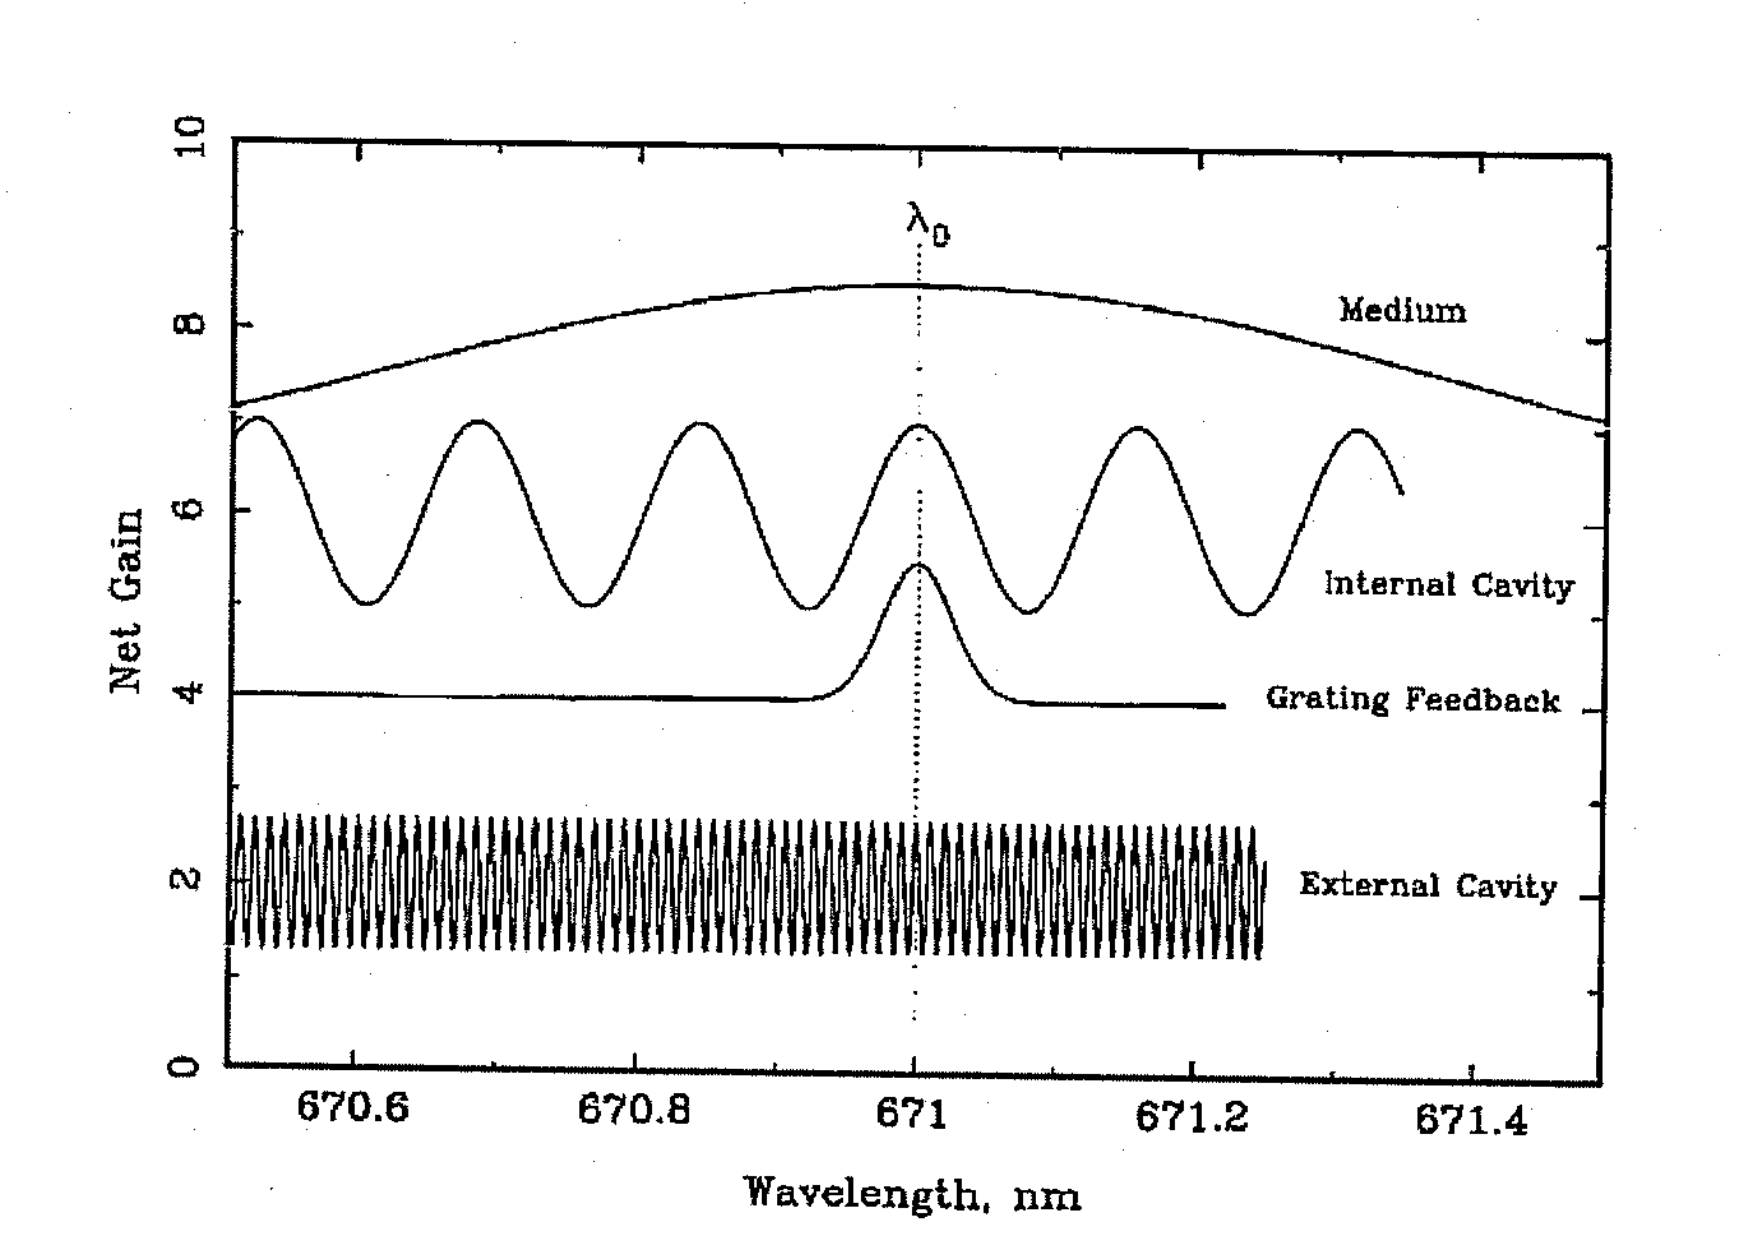
\includegraphics[width=0.7\textwidth]{bilder/contrib.png}
        \caption{Beiträge der einzelnen Beiträge zur Nettoverstärkung.\cite{diodelaserphysics}}
        \label{fig:contrib}
\end{figure}

\begin{figure}[H]
        \centering
        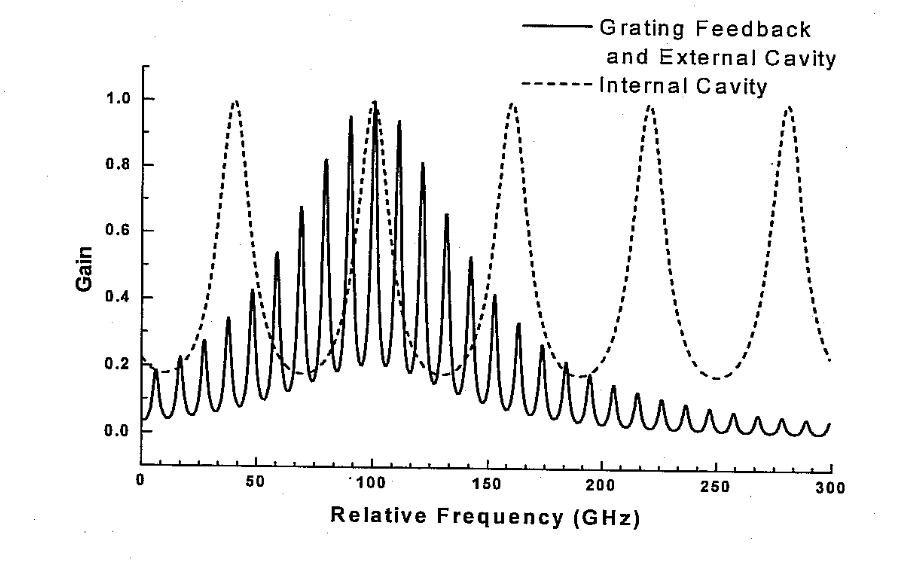
\includegraphics[width=0.7\textwidth]{bilder/int_vs_git_ext.png}
        \caption{Beiträge von Gitter und externem Resonator in Überlagerung mit dem Beitrag des internen Resonators .\cite{diodelaserphysics}}
        \label{fig:int_vs_git_ext}
\end{figure}

Begründet durch die Verteilung der Maxima der einzelnen Verstärkungsbeiträge kann es zu Modensprüngen kommen, also dem abrupten Frequenzwechsel
des Laserlichtes. \autoref{fig:modeshift} zeigt ebensolche unter Änderung des Gitterwinkels, wobei wieder der Beitrag der Gitterrückkopplung und des externen Resonators kombiniert und des
internen Resonators dargestellt sind.

\begin{figure}[H]
        \centering
        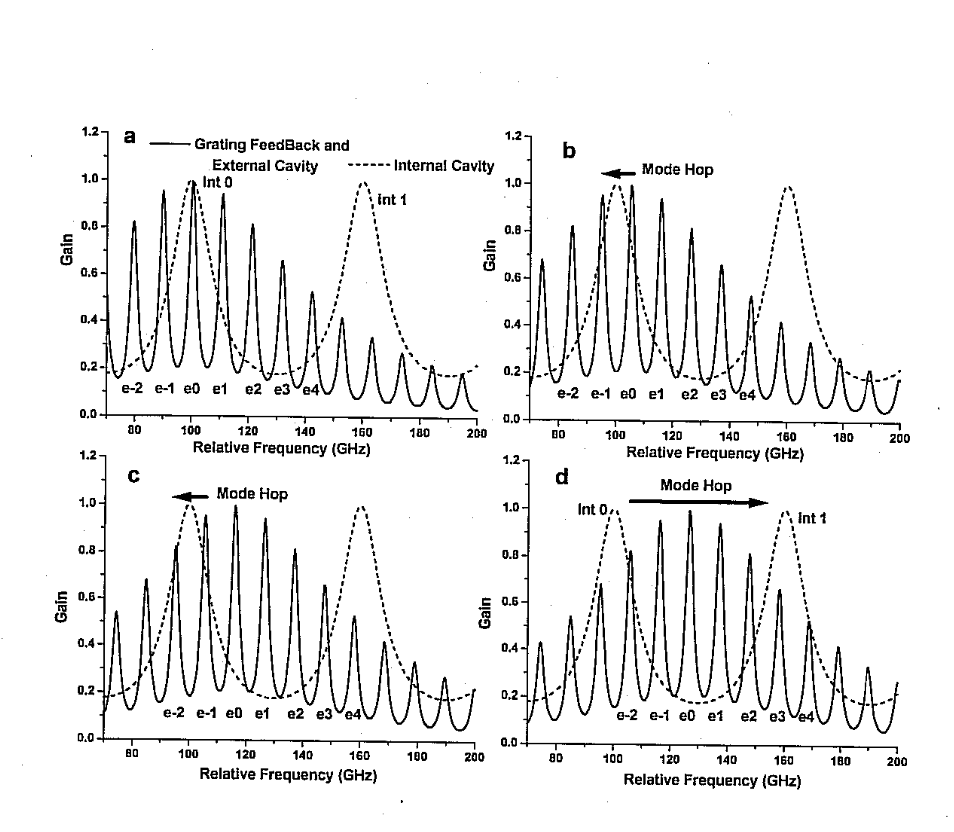
\includegraphics[width=0.7\textwidth]{bilder/modeshift.png}
        \caption{Modensprünge in Abhängigkeit von Gitterwinkeländerungen.\cite{diodelaserphysics}}
        \label{fig:modeshift}
\end{figure}



\subsection{Hyperfeinstrukturübergänge von Rubidium und Transmissionsspektrum}

Als Hyperfeinstruktur wird die Aufspaltung atomarer Energieniveaus durch Kopplung des magnetischen Kernmomentes mit dem magnetischen Moment der Hüllelektronen am Kernort
bezeichnet. So bewirkt die Kopplung von Hüllendrehimpuls und Kernspin eine Quantisierung des Gesamtdrehimpulses und damit in einem externen magnetfeld eine diskrete Aufspaltung von 
Absorptions- und damit Transmissionslinien.\cite{chemie_hfs}
An- und Abregungen dieser Energieniveaus werden als Hyperfeinstrukturübergänge des Atoms bezeichnet.
Das in diesem Versuch untersuchte Rubidium ist ein Isotopengemisch aus $^{85}\mathrm{Rb}$ und $^{87}\mathrm{Rb}$ und besitzt imsgesamt 4 opische atomare Übergänge
im betrachteten Bereich. Die untersuchten Rubidium-Hyperfeinstrukturübergänge, sowie deren Transmissionsminima in Abhängigkeit der Energie sind in \autoref{fig:rb_trans} dargestellt.


\begin{figure}[H]
        \centering
        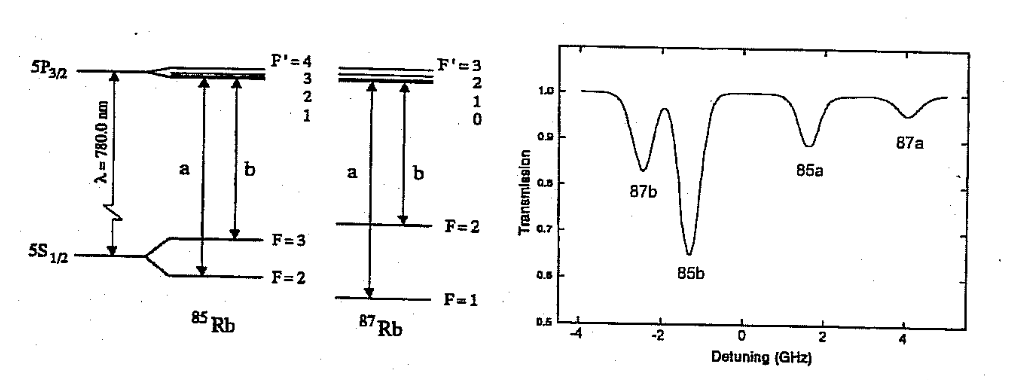
\includegraphics[width=0.7\textwidth]{bilder/rb_trans.png}
        \caption{Betrachtete Hyperfeinstrukturübergänge von Rubidium.\cite{diodelaserphysics}}
        \label{fig:rb_trans}
\end{figure}








\section{Versuchsaufbau}

\autoref{fig:aufbau_numm} zeigt anhand eines selbstgeschossenen Fotos den verwendeten Versuchsaufbau.

\begin{figure}[H]
        \centering
        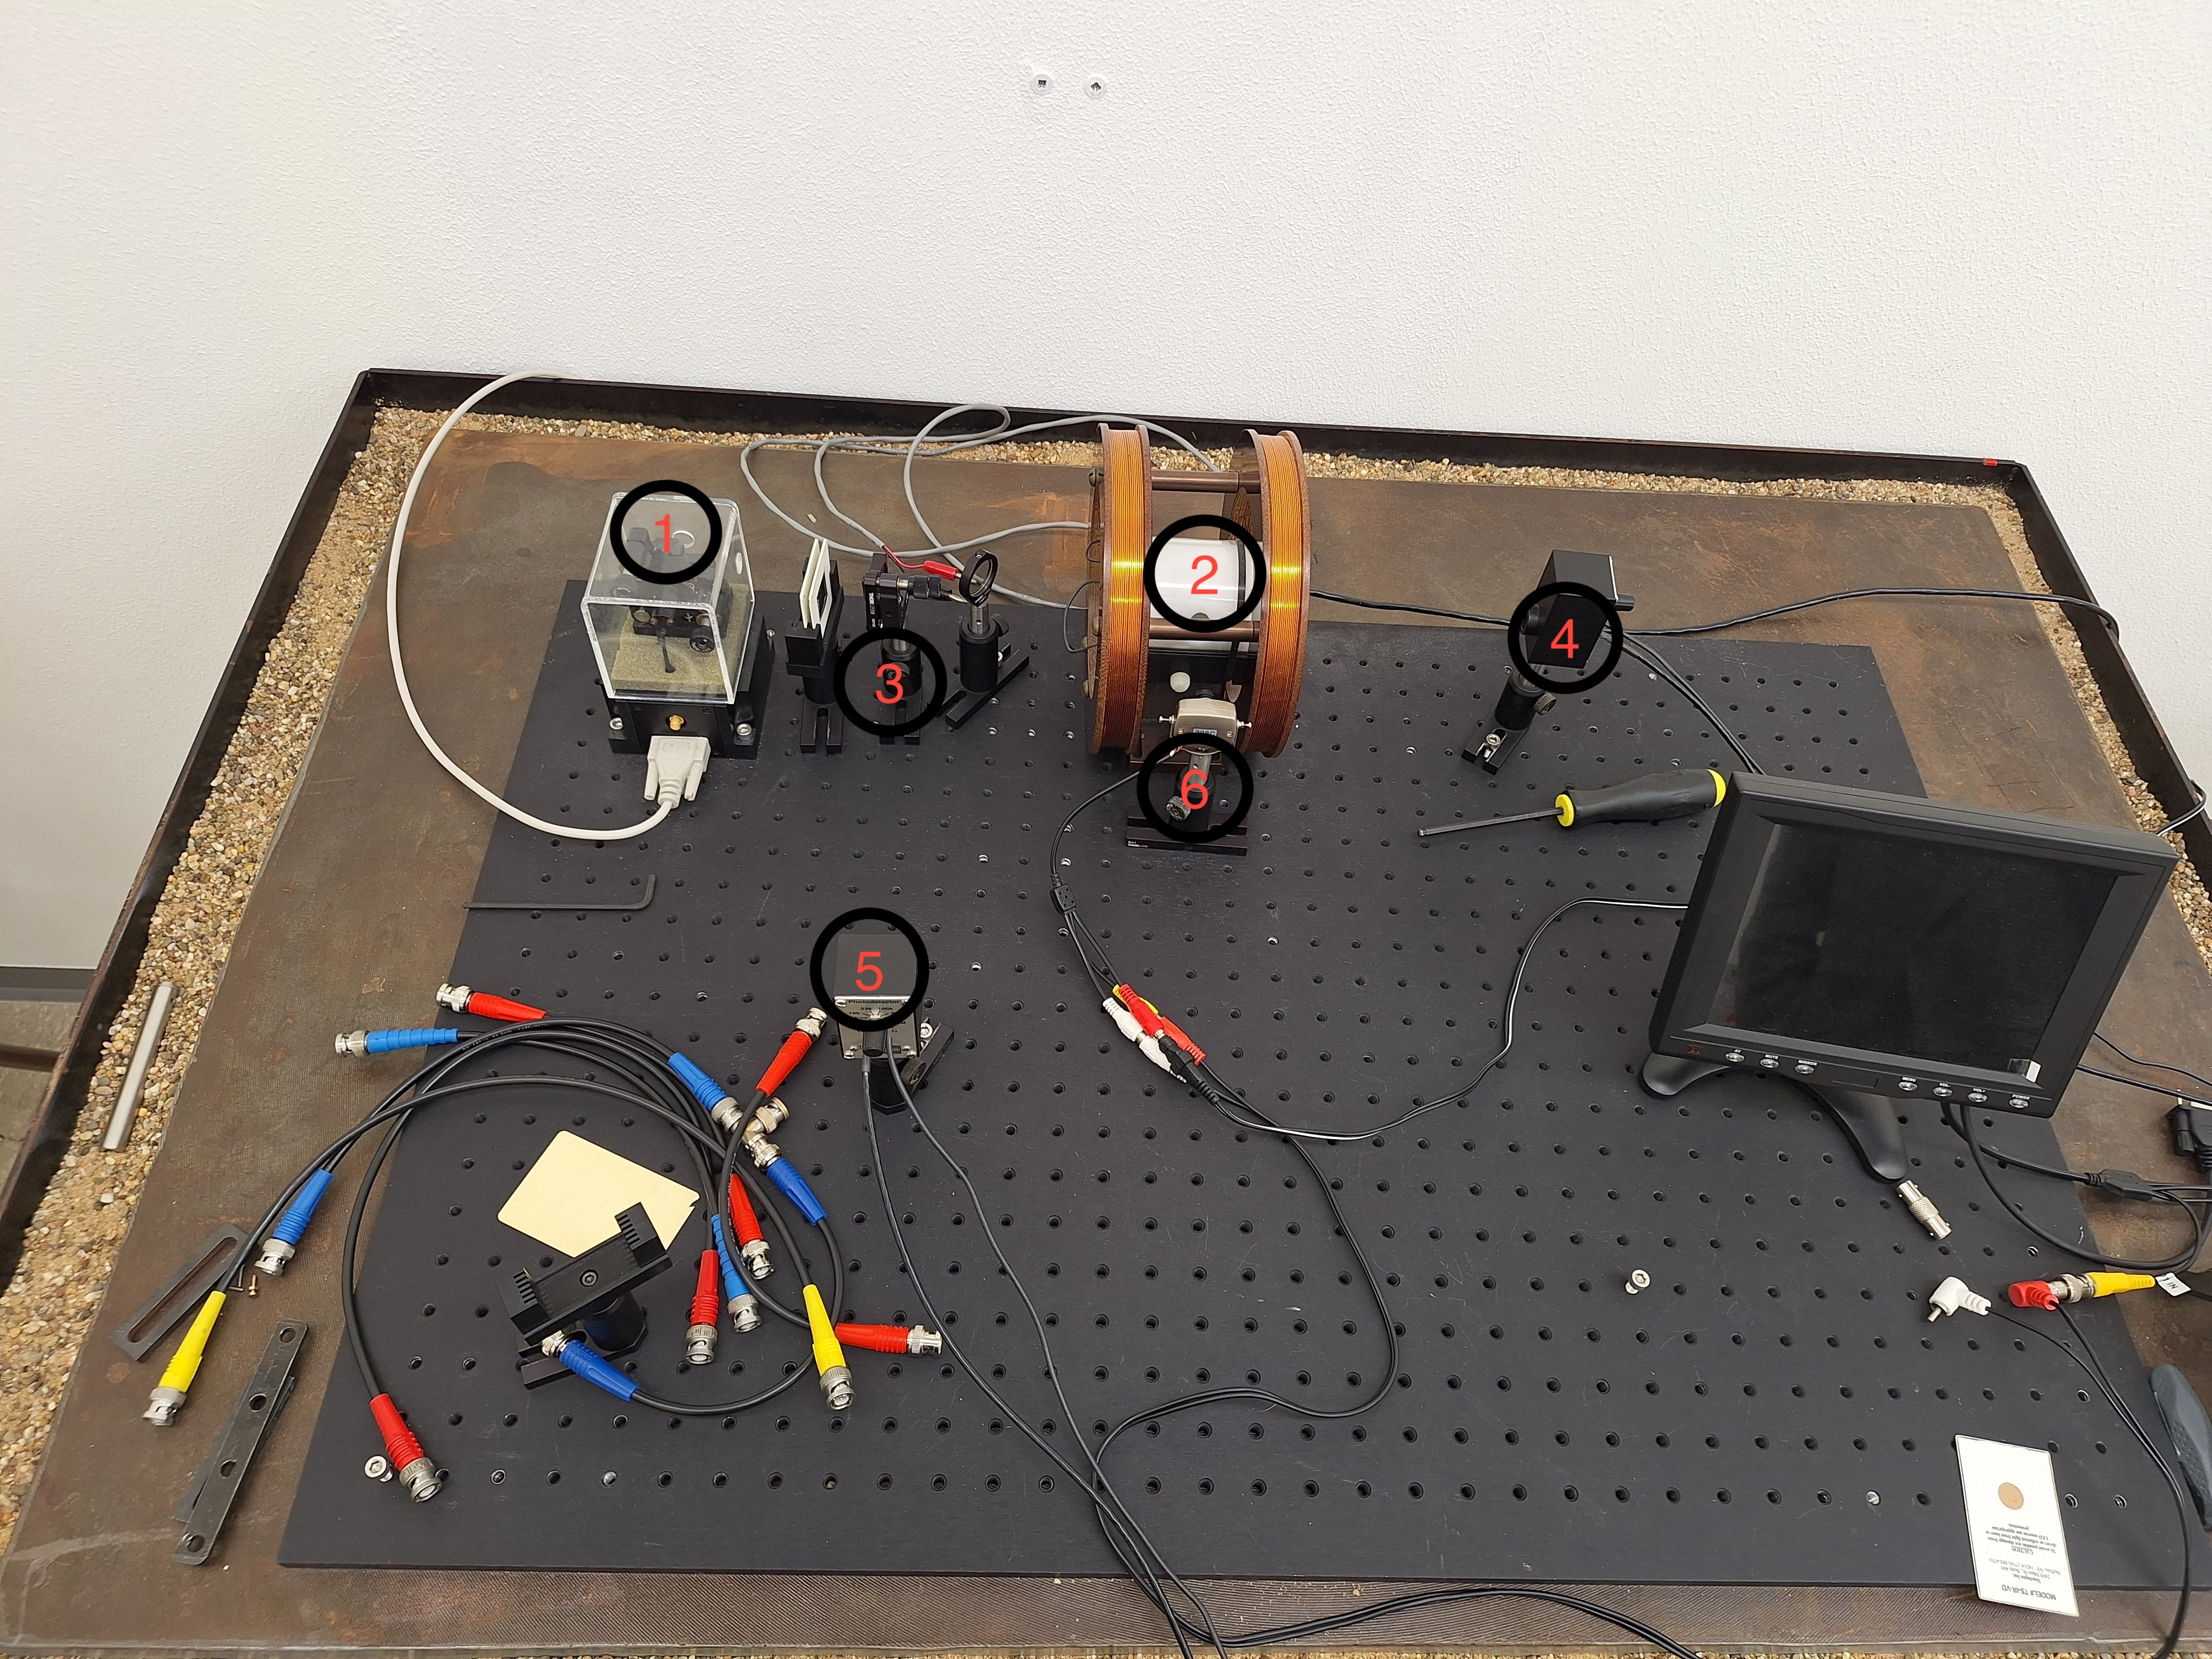
\includegraphics[width=0.8\textwidth]{bilder/aufbau_numm.jpg}
        \caption{Verwendeter Versuchsaufbau.}
        \label{fig:aufbau_numm}
\end{figure}


(1) zeigt die mit dem Littrow-Gitter kombinierte Laserdiode, der Winkel des Gitters gegenüber der Austrittsöffnung des Lasers kann über am Rahmen 
angebrachte Stellschrauben variiert werden kann.
Die Rubidiumzelle mit Fensterung (2) ist von einer Helmholtzspule umgeben, vor dem Fenster ist die Kamera (6) zur Aufnahme der Fluoreszenzlinie
des Rubidiums positioniert.
(3) zeigt die Stative von Laserkarte, Neutraldichtefilter und 50/50-Strahlteiler, die bei betreffenden Abschnitten des Versuchs in den Strahlengang zwischen
Laserdiode und Rubidiumzelle eingebracht werden.
(4) und (5) sind die Photodetektoren, mit deren Hilfe über das Lichtsignal als Spannung in das verwendete Oszilloskop für folgend beschriebene Untersuchungen eingekoppelt
wird.





\section{Durchführung}

In der Versuchsdurchführung werden die Betriebsparameter des Diodenlasers über die Potentiometer am Controller sowie die Detektions- und Oszilloskopeinstellungen schrittweise so abgestimmt, dass die jeweiligen Laserzustände und Absorptionsspektren sauber aufgenommen werden können. Während der gesamten Arbeit mit dem eingeschalteten Laser wird eine Laserschutzbrille getragen und der Raum abgedunkelt.

Zu Beginn werden die Temperaturregelung der Laserdiode sowie die Heizung der Rubidium-Dampfzelle eingeschaltet. Nach Erreichen des thermischen Gleichgewichts wird die Monitor-Spannung $U_T$ am Controller abgelesen, um die Betriebstemperatur des Lasers zu bestimmen.
Anschließend wird der Diodenstrom ausgehend von einem niedrigen Wert schrittweise erhöht, während der Strahl auf einer Karte beobachtet wird. Dabei wird der Übergang vom diffusen, schwachen Leuchten (LED-Betrieb) zum Auftreten eines hellen, klar begrenzten Laserpunkts mit Lasergranulation (Laserbetrieb) abgewartet. Die zugehörige Monitor-Spannung $U_{\text{th}}$ an der Laserschwelle wird notiert und das Strahlprofil vom Bildschirm abfotografiert.

Im kontinuierlichen Laserbetrieb oberhalb der Schwelle wird die Kamera auf die beheizte Rubidiumzelle gerichtet und diese über den Bildschirm beobachtet. Durch leichtes Justieren des Beugungsgitters mithilfe eines Inbusschlüssels sowie durch Verstellen der Piezospannung und bei Bedarf des Diodenstroms wird die Laserfrequenz variiert, bis entlang des Strahlengangs in der Zelle eine deutliche Fluoreszenzlinie sichtbar wird. Die entsprechende Piezospannung $U_{\text{Piezo}}$ wird abgelesen und die Linie fotografiert.

Für die Absorptionsspektroskopie steht ein ND-Filter zwischen Laser und Rubidiumzelle. Eine Photodiode hinter der Zelle wird mit dem Oszilloskop verbunden. Um einen ausreichend großen, modensprungfreien Frequenzbereich abzufahren, werden Diodenstrom und Piezospannung gleichzeitig mit einem Dreieckssignal moduliert. Durch schrittweises Nachregeln der Potentiometer für Rampenamplitude, Offset und Diodenstrom werden die Einstellungen so lange optimiert, bis alle vier Rubidium-Absorptionslinien vollständig sichtbar sind. Von dieser Einstellung werden sowohl eine Oszilloskop-Aufnahme als auch die Rohdaten als CSV-Datei gespeichert.

In einem zweiten Durchgang werden das Piezo-Monitorsignal auf Channel~1 und das Photodiodensignal auf Channel~2 des Oszilloskops gelegt, sodass beide Signale synchron aufgezeichnet und wieder als Bild und CSV-Datei gesichert werden können.

Abschließend wird für die Differenzmessung eine zweite Photodiode über einen $50/50$-Strahlteiler als Referenz in den Strahlengang eingebracht. Die Photodiode hinter der Zelle (PD~1) wird an den $(+)$-Eingang und die Referenz-Photodiode (PD~2) an den $(-)$-Eingang angeschlossen. Über die Balance-Potentiometer wird die Differenz beider Signale so abgeglichen, dass der linear ansteigende Untergrund möglichst flach verläuft. Das resultierende Absorptionsspektrum mit den vier Absorptionsminima wird erneut als Oszilloskop-Aufnahme und CSV-Datensatz gespeichert.

\section{Auswertung}

Die Auswertung, die Fits sowie die Erstellung der Diagramme wurden mit Python mit den Bibliotheken \texttt{NumPy}, \texttt{SciPy} und \texttt{Matplotlib} durchgeführt. Die Unsicherheiten aller abgeleiteten Größen wurden mithilfe der Gauß'schen Fehlerfortpflanzung berechnet
\begin{equation*}
    \sigma_f = \sqrt{\sum_{i} \left(\frac{\partial f}{\partial x_i}\,\sigma_{x_i}\right)^2}.
\end{equation*}

\subsection{Temperaturregelung des Lasers}
\label{subsec:temperatur}

Die Emissionswellenlänge einer Laserdiode ist stark temperaturabhängig. Es wurde eine Spannung von $U_T = \SI{1.97}{\volt}$ abgelesen. Durch lineare Interpolation 
\begin{equation*}
T_{\text{Laser}} = T_1 + \frac{U_T - U_1}{U_2 - U_1}\,(T_2 - T_1)
= \SI{35}{\degreeCelsius} + \frac{\SI{1.97}{\volt} - \SI{1.9756}{\volt}}{\SI{1.9269}{\volt} - \SI{1.9756}{\volt}}\,(\SI{36}{\degreeCelsius} - \SI{35}{\degreeCelsius}) \approx \SI{35.11}{\degreeCelsius}
\end{equation*}
erhalten wir eine Betriebstemperatur von $T_{\text{Laser}} \approx \SI{35.1}{\degreeCelsius}$. Die Rubidiumzelle wurde zur Erhöhung der Dampfdichte und damit des Signals auf etwa $\SI{50}{\degreeCelsius}$ beheizt.

\subsection{Bestimmung der Laserschwelle}

Zur Bestimmung der Laserschwelle wurde der Strom der Laserdiode schrittweise erhöht und das Strahlprofil beobachtet. Unterhalb der Schwelle emittiert die Diode lediglich schwache, spontane Strahlung mit einem breiten, diffusen Profil (LED-Betrieb). Bei einer Monitor-Spannung von $U_{\text{th}} = \SI{0.19}{\volt}$ setzt die stimulierte Emission ein und die Intensität steigt sprunghaft an und es bildet sich ein klar begrenzter Laserpunkt mit Lasergranulation (Laserbetrieb, siehe Abbildung~\ref{fig:lasermodus}).

\begin{figure}[htbp]
    \centering
    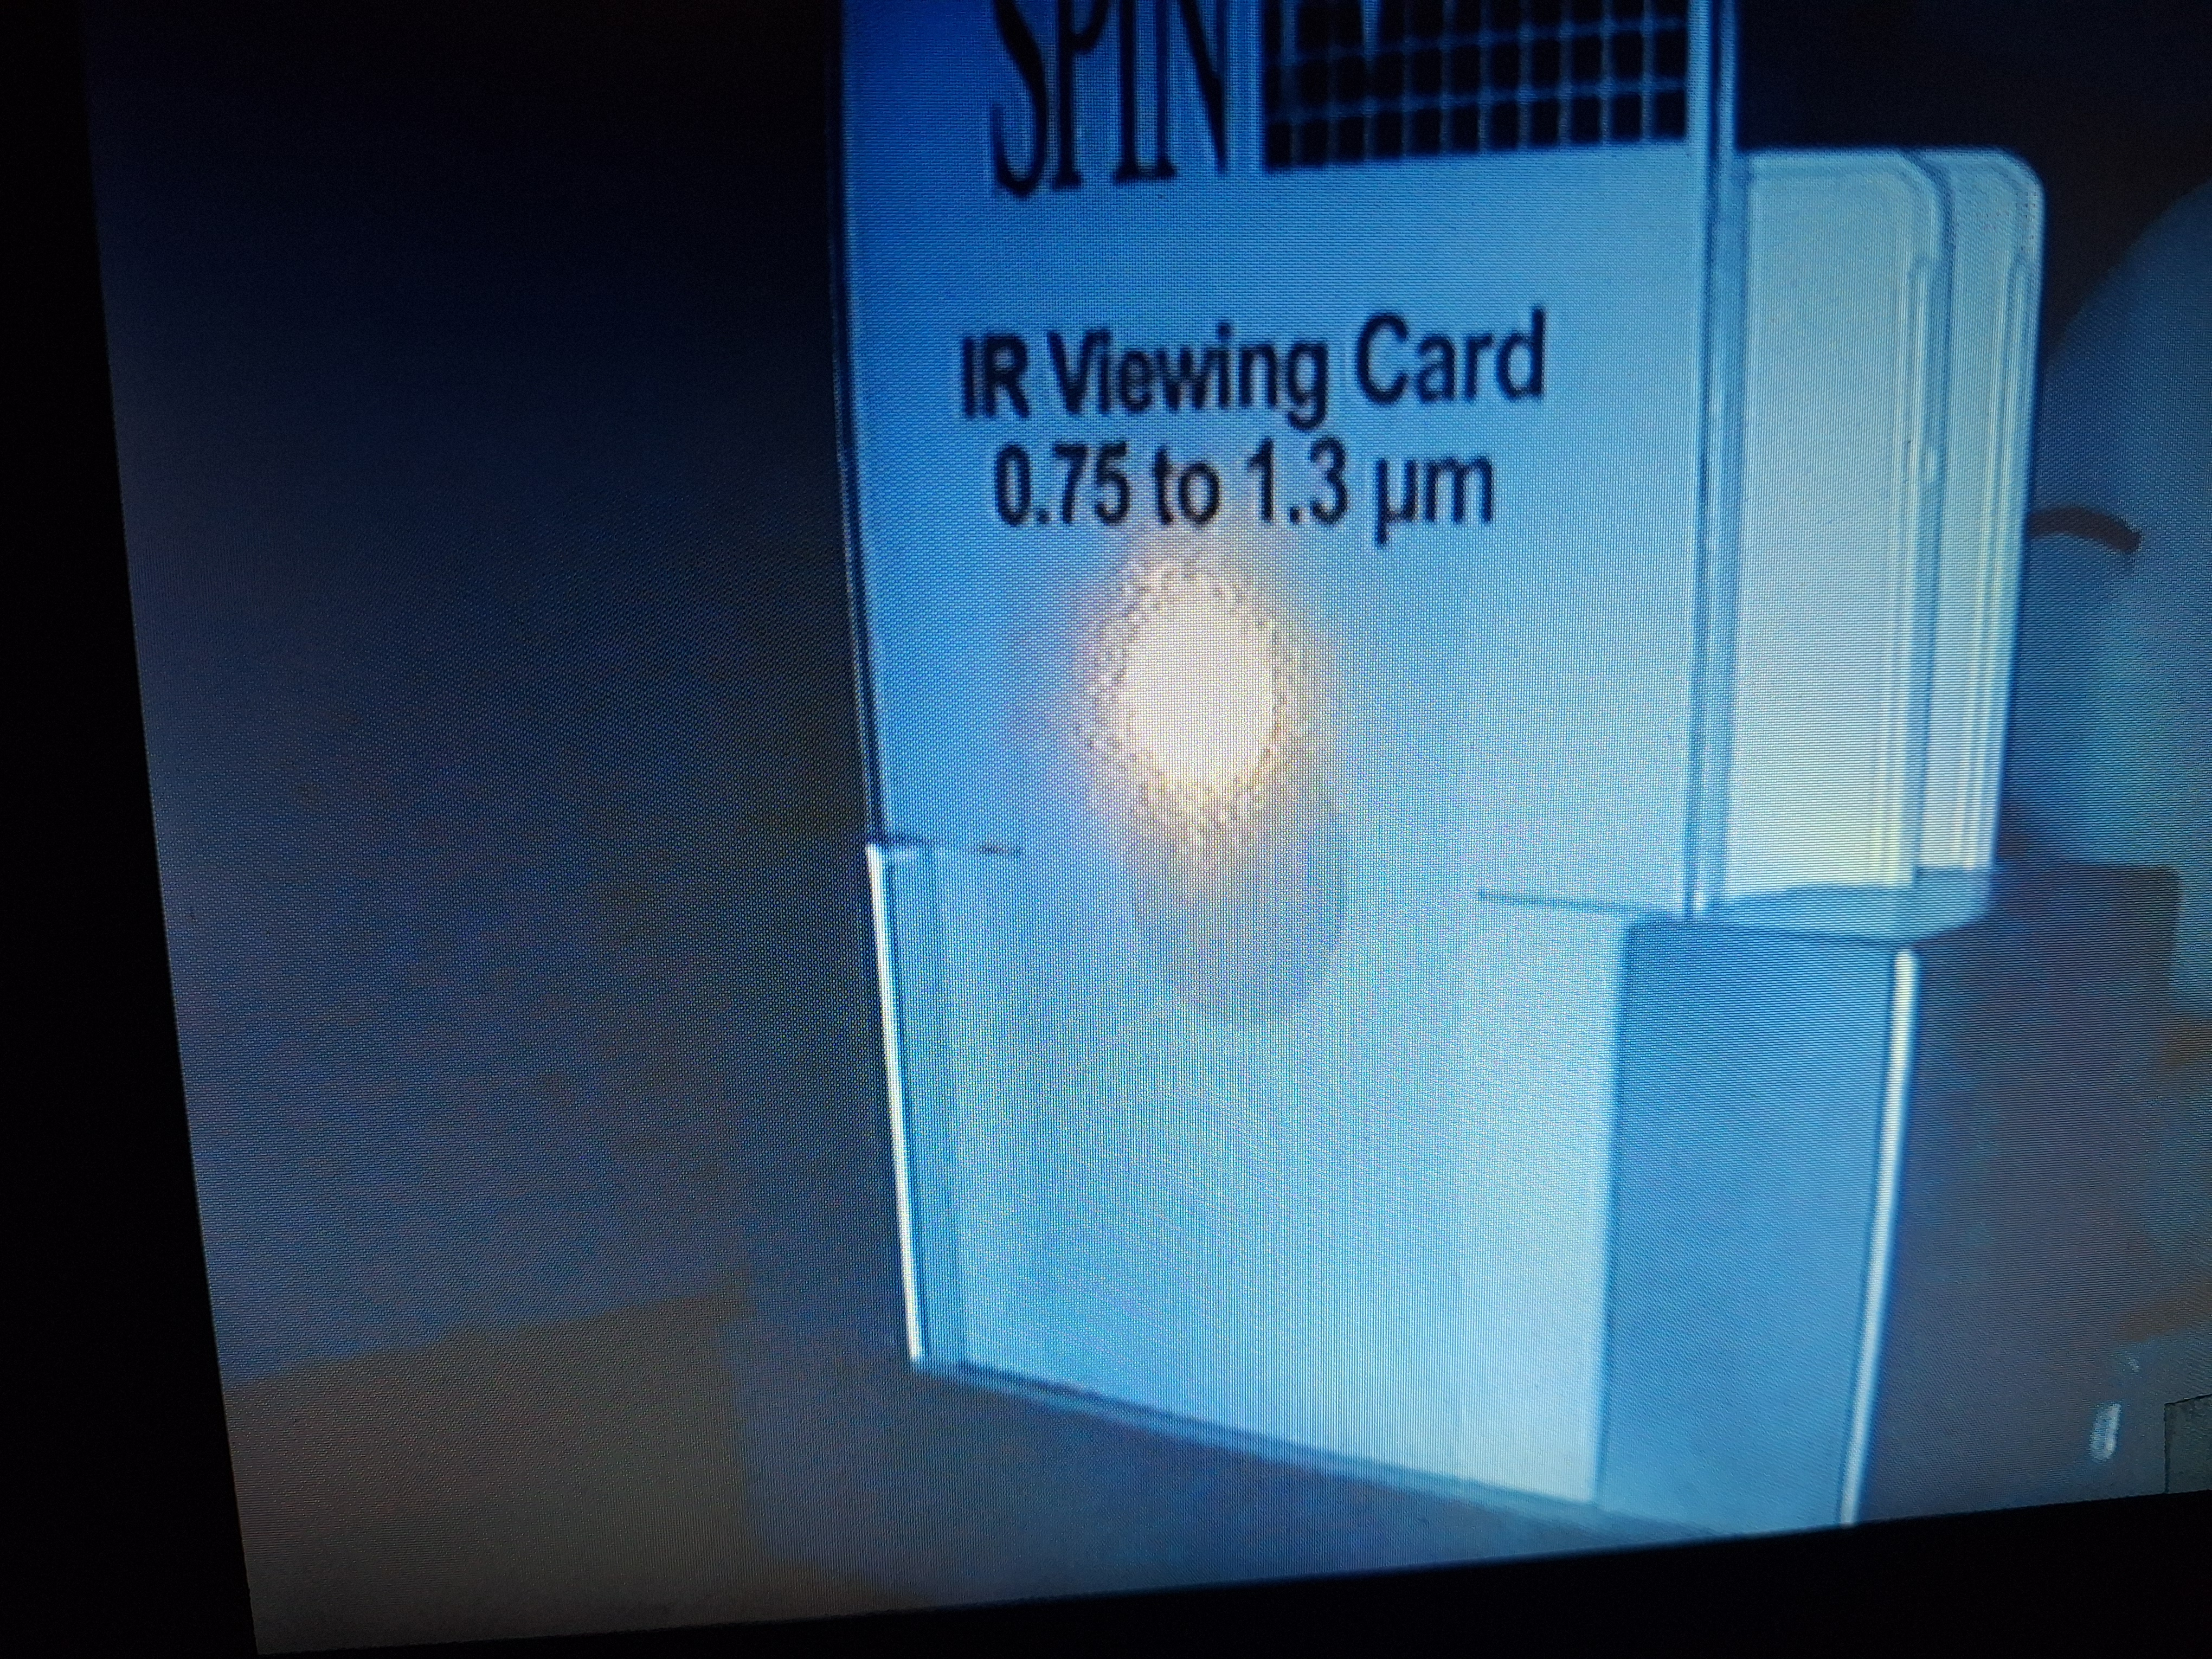
\includegraphics[width=0.65\textwidth]{bilder/lasermodus.jpg}
    \caption{Aufnahme des gebündelten Strahlprofils auf der Betrachtungskarte oberhalb der Laserschwelle im Laserbetrieb.}
    \label{fig:lasermodus}
\end{figure}

\subsection{Rubidium-Fluoreszenz}

Um den Laser auf die Rubidium-$D_2$-Linie bei $\lambda = \SI{780.241}{\nano\meter}$\footnote{P. Siddons et al., J. Phys. B \textbf{41}, 155004 (2008), Kap.~2.4.} abzustimmen, wurde die Piezospannung am Beugungsgitter im kontinuierlichen Laserbetrieb variiert, während die beheizte Rubidiumzelle beobachtet wurde. Bei einer eingestellten Spannung von $U_{\text{Piezo}} = \SI{6.67}{\volt}$ trat eine deutliche, leicht flackernde Fluoreszenzlinie entlang des Laserstrahls in der Zelle auf (Abbildung~\ref{fig:rb_linie}). Dies zeigt, dass die Laserfrequenz resonant mit einem der atomaren Übergänge des Rubidiums ist und die angeregten Atome das absorbierte Licht spontan in alle Raumrichtungen abstrahlen.

\begin{figure}[htbp]
    \centering
    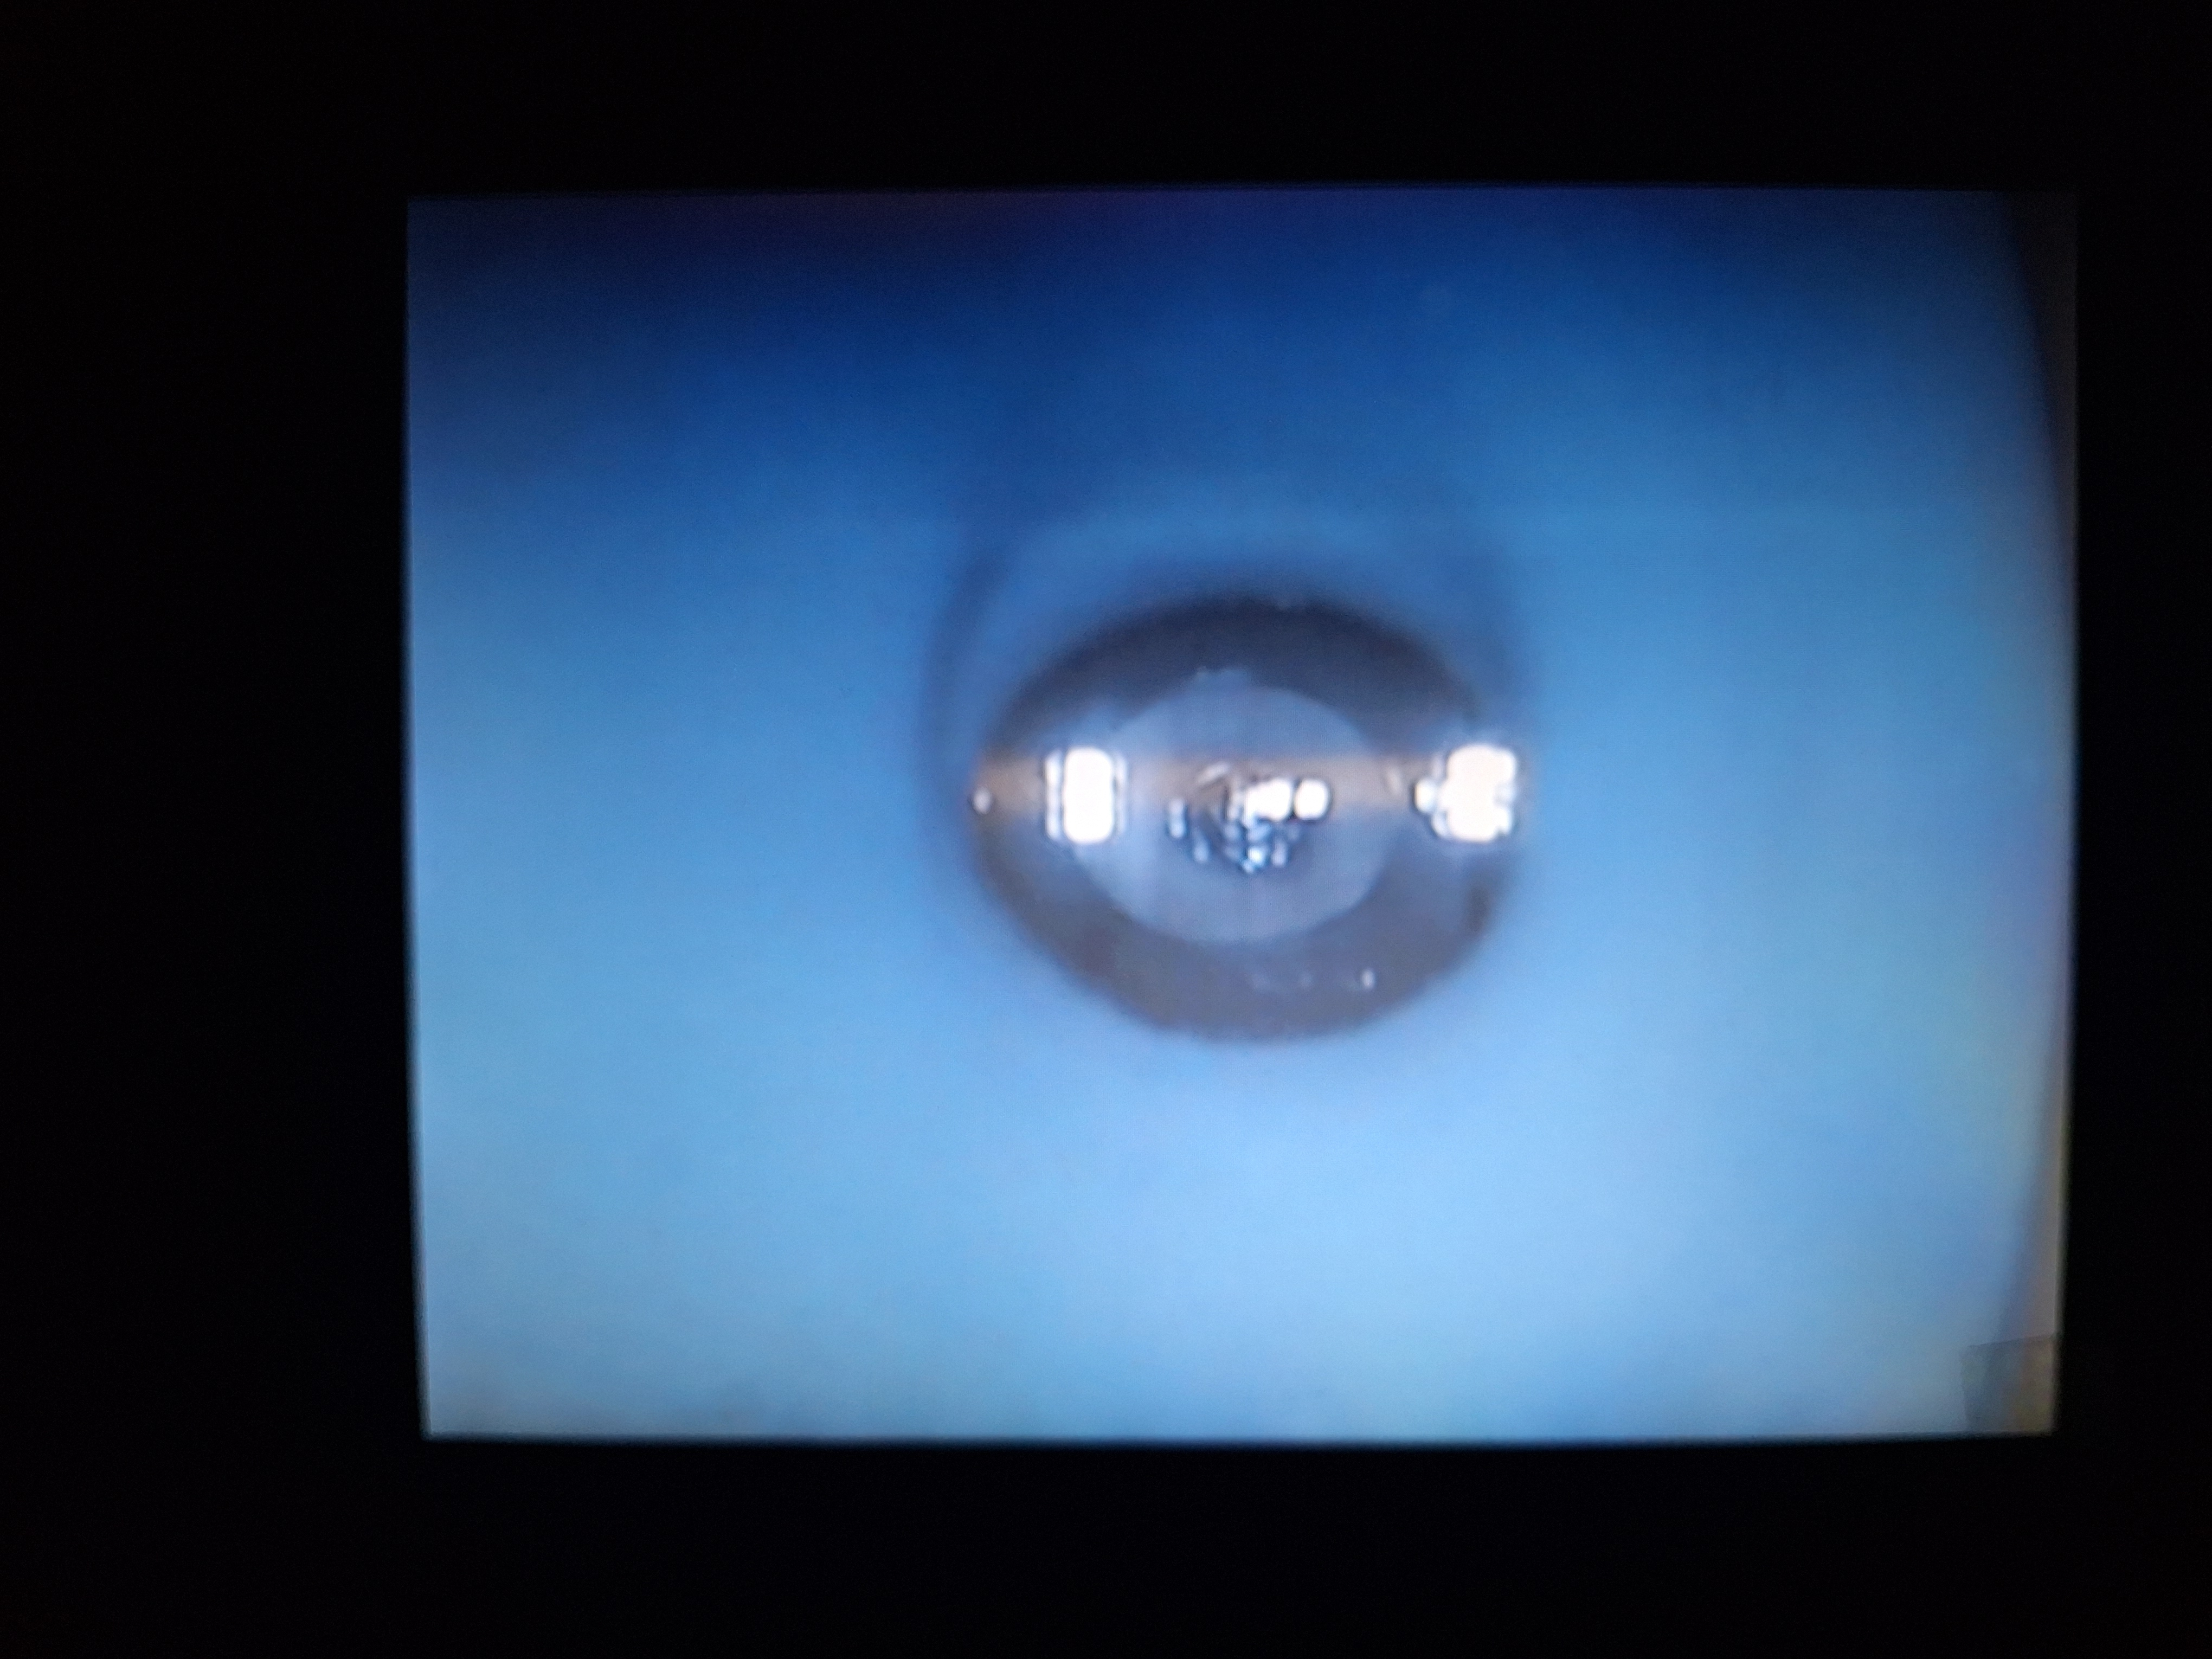
\includegraphics[width=0.72\textwidth]{bilder/rb-Linie.jpg}
    \caption{Aufnahme der Rubidiumlinie in der Dampfzelle}
    \label{fig:rb_linie}
\end{figure}

\subsection{Absorptionsspektrum (1 PD)}

Durch gleichzeitiges periodisches Variieren von Diodenstrom und Piezospannung lässt sich ein modensprungfreier Frequenzbereich abfahren, der alle vier Absorptionslinien des Rubidiums abdeckt. Abbildung~\ref{fig:1pd_oszi} zeigt die zugehörige Aufnahme direkt vom Oszilloskop.

\begin{figure}[htbp]
    \centering
    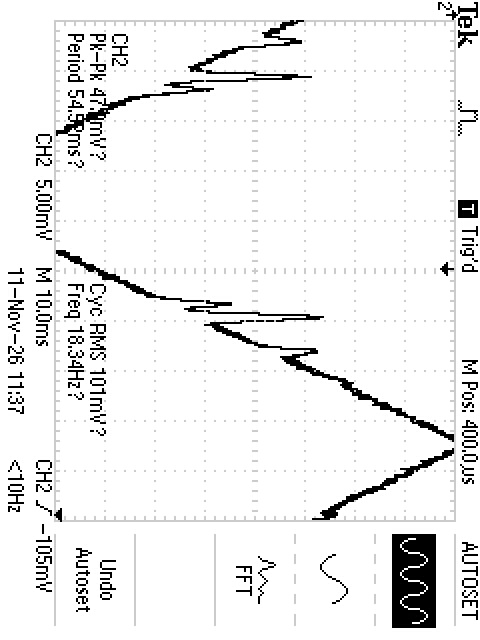
\includegraphics[angle=90, width=0.65\textwidth]{bilder/F0017TEK.jpg}
    \caption{Oszilloskop-Aufnahme des Rubidium-Absorptionsspektrums mit einer Photodiode.}
    \label{fig:1pd_oszi}
\end{figure}

Aus den zugehörigen Oszilloskop-Daten lassen sich alle vier charakteristischen Übergänge der Isotope $^{85}\text{Rb}$ mit natürlicher Häufigkeit von $\SI{72.17}{\percent}$ und $^{87}\text{Rb}$ mit $\SI{27.83}{\percent}$\footnote{P. Siddons, C. S. Adams, C. Ge und I. G. Hughes, \textit{Absolute absorption on rubidium D lines: comparison between theory and experiment}, J. Phys. B: At. Mol. Opt. Phys. \textbf{41}, 155004 (2008), Appendix~A.} ablesen

$^{87}\text{Rb}$ b bei $t = \SI{7.04}{\milli\second}$ ($\approx \SI{6.36}{\milli\volt}$)
$^{85}\text{Rb}$ b bei $t = \SI{9.96}{\milli\second}$ ($\approx \SI{12.47}{\milli\volt}$)
$^{85}\text{Rb}$ a bei $t = \SI{16.36}{\milli\second}$ ($\approx \SI{4.90}{\milli\volt}$)
$^{87}\text{Rb}$ a bei $t = \SI{22.16}{\milli\second}$ ($\approx \SI{1.75}{\milli\volt}$)


Die Zuordnung folgt einerseits aus dem charakteristischen Intensitätsmuster und zum anderen aus den relativen Zeitabständen der Linien. Für die Grundzustandsaufspaltungen ergeben sich Zeitdifferenzen von $\Delta t(^{85}\text{Rb}) = \SI{6.40}{\milli\second}$ zwischen 85b und 85a sowie $\Delta t(^{87}\text{Rb}) = \SI{15.12}{\milli\second}$ zwischen 87b und 87a. Das Verhältnis beträgt
\begin{equation*}
    \frac{\Delta t(^{87}\text{Rb})}{\Delta t(^{85}\text{Rb})} = \frac{\SI{15.12}{\milli\second}}{\SI{6.40}{\milli\second}} \approx \num{2.36}.
\end{equation*}

\subsection{Absorptionsspektrum (1 PD) mit Piezo-Monitor}

In der nächsten Messung mit höherem Photodioden-Gain wurden beide Kanäle des Oszilloskops gleichzeitig aufgezeichnet. Abbildung~\ref{fig:1pd_ch12_oszi} zeigt die direkte Oszilloskop-Aufnahme.

\begin{figure}[htbp]
    \centering
    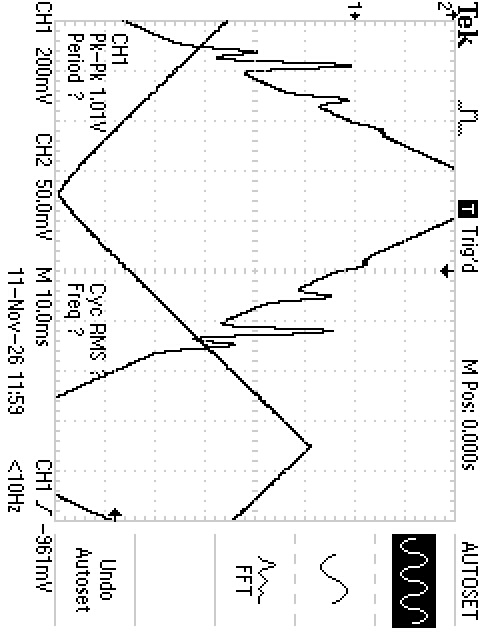
\includegraphics[angle=90, width=0.65\textwidth]{bilder/F0018TEK.jpg}
    \caption{Oszilloskop-Aufnahme des 1-PD-Absorptionsspektrums zusammen mit dem Piezo-Monitorsignal.}
    \label{fig:1pd_ch12_oszi}
\end{figure}

Channel~1 zeigt das $\SI{10}{\hertz}$-Dreieckssignal des Piezo Monitor Output, linear ansteigend von $\approx \SI{-1.0}{\volt}$ bis $\approx \SI{-0.2}{\volt}$. Channel~2 gibt die negative Ausgangsspannung der Photodiode hinter der Rubidiumzelle wieder, wobei die strombedingte Leistungszunahme den linear abfallenden Untergrund erzeugt und die vier Peaks den Rubidium-Absorptionslinien entsprechen.
Auf der steigenden Flanke der Piezorampe durchläuft der Laser die Frequenzen in umgekehrter Richtung, sodass die vier Linien von links nach rechts in der Reihenfolge $^{87}\text{Rb}$~a, $^{85}\text{Rb}$~a, $^{85}\text{Rb}$~b und $^{87}\text{Rb}$~b erscheinen. Aus den zugehörigen CSV-Daten ergeben sich die Positionen:

$^{87}\text{Rb}$ a bei $t = \SI{9.36}{\milli\second}$ ($\approx \SI{16.09}{\milli\volt}$)
$^{85}\text{Rb}$ a bei $t = \SI{15.20}{\milli\second}$ ($\approx \SI{49.02}{\milli\volt}$)
$^{85}\text{Rb}$ b bei $t = \SI{22.28}{\milli\second}$ ($\approx \SI{129.74}{\milli\volt}$)
$^{87}\text{Rb}$ b bei $t = \SI{25.04}{\milli\second}$ ($\approx \SI{62.43}{\milli\volt}$)


Für die Grundzustandsaufspaltungen sind die Zeitdifferenzen $\Delta t(^{85}\text{Rb}) = \SI{7.08}{\milli\second}$ und $\Delta t(^{87}\text{Rb}) = \SI{15.68}{\milli\second}$. Das Verhältnis beträgt
\begin{equation*}
    \frac{\Delta t(^{87}\text{Rb})}{\Delta t(^{85}\text{Rb})} = \frac{\SI{15.68}{\milli\second}}{\SI{7.08}{\milli\second}} \approx \num{2.21}.
\end{equation*}\subsection{Absorptionsspektrum (2 PD)}

Um den Untergrund zu entfernen, wurde im letzten Versuchsteil eine zweite Photodiode über einen $50/50$-Strahlteiler in den Strahlengang eingebracht. Durch Subtraktion beider Photodiodensignale entsteht ein nahezu konstanter Untergrund bei $\approx \SI{331}{\milli\volt}$ mit vier deutlichen Absorptionsminima. Abbildung~\ref{fig:2pd_oszi} zeigt die direkte Oszilloskop-Aufnahme dieser Messung.

\begin{figure}[htbp]
    \centering
    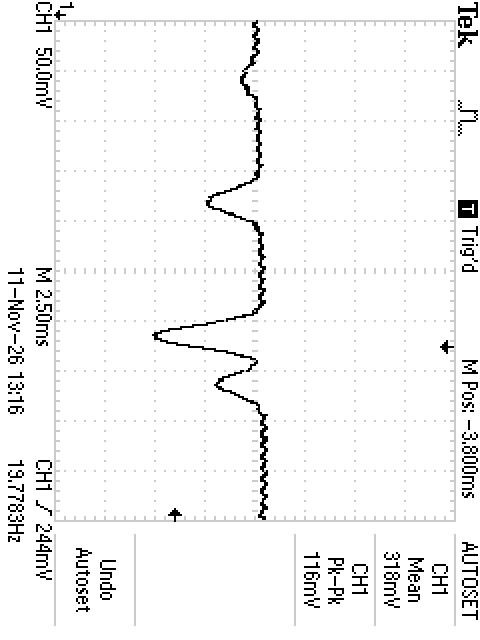
\includegraphics[angle=90, width=0.65\textwidth]{bilder/F0019TEK.jpg}
    \caption{Oszilloskop-Aufnahme des Rubidium Absorptionsspektrums mit zwei Photodioden (Differenzmessung).}
    \label{fig:2pd_oszi}
\end{figure}

\subsubsection{Kalibrierung der Frequenzachse}

Das Oszilloskop zeichnet die Differenzspannung der beiden Photodioden zunächst als Funktion der Zeit $t$ auf. Um die $x$-Achse von einer willkürlichen Zeitachse (in $\si{\milli\second}$) in eine physikalisch aussagekräftige Frequenzverstimmung $\Delta\nu$ (in $\si{\giga\hertz}$) umzurechnen, werden die vier Rubidium-Absorptionslinien selbst als Referenzmaßstab genutzt. Die zugehörigen Literaturfrequenzen der vier $D_2$-Linien, bezogen auf den gemeinsamen Schwerpunkt bei $\SI{384230426.6}{\mega\hertz}$ wurden jeweils über die Übergangsstärken gemittelt\footnote{Berechnet aus den tabellierten $D_2$-Übergangsfrequenzen und Übergangsstärken in P. Siddons et al., J. Phys. B \textbf{41}, 155004 (2008), Table~1(a) und Table~B1.}.

Hierzu wurden zunächst die zeitlichen Positionen $t_i$ der vier Absorptionsminima bestimmt und den jeweiligen Literaturwerten $\Delta\nu_{\text{lit}, i}$ zugeordnet (siehe Tabelle~\ref{tab:kalibrierung}).

\begin{table}[htbp]
    \centering
    \caption{Gemessene Zeitpositionen $t_i$ der vier Rubidium-$D_2$-Linien und die zugehörigen Literaturfrequenzen $\Delta\nu_{\text{lit}, i}$ für die Kalibrierung der $x$-Achse.}
    \label{tab:kalibrierung}
    \begin{tabular}{lcc}
        \toprule
        Übergang & Zeitposition $t_i$ / $\si{\milli\second}$ & Literaturwert $\Delta\nu_{\text{lit}, i}$ / $\si{\giga\hertz}$ \\
        \midrule
        $^{87}\text{Rb}$ a & $\num{-13.343 \pm 0.010}$ & $\num{+4.153}$ \\
        $^{85}\text{Rb}$ a & $\num{-7.208 \pm 0.003}$  & $\num{+1.676}$ \\
        $^{85}\text{Rb}$ b & $\num{-0.500 \pm 0.001}$  & $\num{-1.235}$ \\
        $^{87}\text{Rb}$ b & $\num{+1.917 \pm 0.003}$  & $\num{-2.399}$ \\
        \bottomrule
    \end{tabular}
\end{table}

Unter der Annahme, dass sich die Laserfrequenz während des Scans linear mit der Zeit ändert, wird eine lineare Regression der Form
\begin{equation}
    \Delta\nu(t) = m \cdot t + b
    \label{eq:kalibrierung}
\end{equation}
an die vier Wertepaare angepasst. Die Rechnung liefert die Parameter
\begin{align}
    m &= \SI{-0.4283 \pm 0.0085}{\giga\hertz\per\milli\second}, \\
    b &= \SI{-1.500 \pm 0.065}{\giga\hertz}
\end{align}
mit einem Bestimmtheitsmaß von $R^2 = \num{0.9992}$. Die negative Steigung $m$ ergibt sich daraus, dass die Laserfrequenz auf der betrachteten Flanke abnimmt. Mit Gleichung~\eqref{eq:kalibrierung} lassen sich anschließend alle gemessenen Zeitpunkte direkt in die Frequenzverstimmung $\Delta\nu$ umrechnen, auf deren Grundlage der 4-fach-Gauß-Fit durchgeführt wird.

\subsubsection{4-fach-Gauß-Fit}
Zur quantitativen Auswertung der Absorptionslinien auf der kalibrierten Frequenzachse wird eine Modellfunktion bestehend aus einem linearen Restuntergrund und der Summe von vier negativen Gauß-Funktionen an die Messdaten gefittet
\begin{equation*}
    U(\Delta\nu) = c_0 + c_1 \Delta\nu - \sum_{i=1}^{4} A_i \exp\!\left(-\frac{(\Delta\nu - \mu_i)^2}{2\sigma_i^2}\right).
    \label{eq:four_gauss}
\end{equation*}
Dabei beschreiben $c_0$ und $c_1$ den verbleibenden linearen Untergrund, $A_i$ die jeweilige Absorptionsamplitude, $\mu_i$ die Mittenfrequenz und $\sigma_i$ die Standardabweichung der $i$-ten Linie.

Die Verwendung von Gauß-Profilen ist physikalisch sinnvoll, da die Linienbreite der Rubidium-Übergänge in der auf $\SI{50}{\degreeCelsius}$ beheizten Dampfzelle maßgeblich durch die Dopplerverbreiterung bestimmt wird. Aufgrund der thermischen Bewegung der Atome entsteht ein gaußförmiges Absorptionsprofil mit einer theoretischen Halbwertsbreite von etwa $\SI{530}{\mega\hertz}$. Die natürliche Linienbreite des $D_2$-Übergangs $\Gamma / 2\pi = \SI{6.065}{\mega\hertz}$\footnote{P. Siddons et al., J. Phys. B \textbf{41}, 155004 (2008), Kap.~2.4.} ist dagegen deutlich kleiner und kann vernachlässigt werden. Das eigentliche Voigt-Profil darf durch eine Gauß-Funktion angenähert werden. 
Abbildung~\ref{fig:2pd_fit} zeigt das 2-PD-Spektrum zusammen mit dem angepassten 4-fach-Gauß-Fit. Die Ergebnisse des Fits stehen zusammen mit den berechneten Halbwertsbreiten ($\text{FWHM}_i = 2\sqrt{2\ln 2}\,\sigma_i$) und Peakflächen ($F_i = A_i \sigma_i \sqrt{2\pi}$) in Tabelle~\ref{tab:fit_results}.

\begin{figure}[htbp]
    \centering
    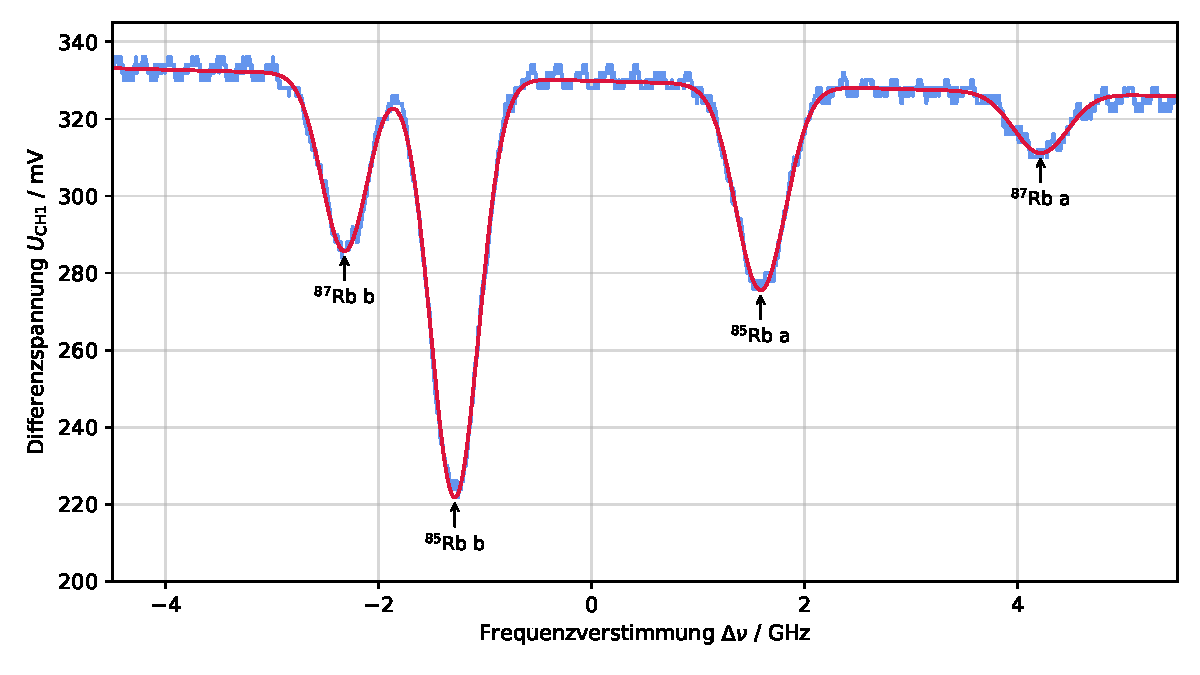
\includegraphics[width=0.85\textwidth]{2PD_spektrum_fit.pdf}
    \caption{Absorptionsspektrum (2 PD) mit 4-fach-Gauß-Fit (rot) und Zuordnung der vier Rubidium-Übergänge.}
    \label{fig:2pd_fit}
\end{figure}

\begin{table}[htbp]
    \centering
    \caption{Ergebnisse des 4-fach-Gauß-Fits an das kalibrierte 2-PD-Absorptionsspektrum.}
    \label{tab:fit_results}
    \begin{tabular}{lcccc}
        \toprule
        Übergang & $\mu_i$ / $\si{\giga\hertz}$ & $A_i$ / $\si{\milli\volt}$ & $\text{FWHM}_i$ / $\si{\mega\hertz}$ & Fläche $F_i$ / $\si{\milli\volt\giga\hertz}$ \\
        \midrule
        $^{87}\text{Rb}$ b & $\num{-2.321 \pm 0.001}$ & $\num{45.88 \pm 0.25}$ & $\num{499.6 \pm 3.2}$ & $\num{24.40 \pm 0.14}$ \\
        $^{85}\text{Rb}$ b & $\num{-1.286 \pm 0.001}$ & $\num{109.03 \pm 0.24}$ & $\num{530.3 \pm 1.4}$ & $\num{61.54 \pm 0.15}$ \\
        $^{85}\text{Rb}$ a & $\num{+1.587 \pm 0.001}$ & $\num{53.15 \pm 0.24}$ & $\num{547.0 \pm 2.9}$ & $\num{30.95 \pm 0.15}$ \\
        $^{87}\text{Rb}$ a & $\num{+4.214 \pm 0.004}$ & $\num{15.67 \pm 0.23}$ & $\num{597.0 \pm 10.8}$ & $\num{9.96 \pm 0.18}$ \\
        \bottomrule
    \end{tabular}
\end{table}

\subsubsection{Bestimmung des Isotopenverhältnisses}
Wir wissen, dass die Fläche unter den jeweiligen Peaks im Bereich geringer optischer Dichte proportional zur Teilchendichte des jeweiligen Isotops ist und so lässt sich das natürliche Isotopenverhältnis von $^{85}\text{Rb}$ zu $^{87}\text{Rb}$ direkt über die Summe der zugehörigen Fitflächen bestimmen mit
\begin{align}
    F(^{85}\text{Rb}) &= F_{85\text{b}} + F_{85\text{a}} = \SI{92.49 \pm 0.21}{\milli\volt\giga\hertz}, \\
    F(^{87}\text{Rb}) &= F_{87\text{b}} + F_{87\text{a}} = \SI{34.36 \pm 0.23}{\milli\volt\giga\hertz}.
\end{align}
Daraus ergeben sich die relativen Häufigkeiten der beiden Isotope zu
\begin{align}
    p(^{85}\text{Rb}) &= \frac{F(^{85}\text{Rb})}{F(^{85}\text{Rb}) + F(^{87}\text{Rb})} = \SI{72.91 \pm 0.14}{\percent}, \\
    p(^{87}\text{Rb}) &= \frac{F(^{87}\text{Rb})}{F(^{85}\text{Rb}) + F(^{87}\text{Rb})} = \SI{27.09 \pm 0.14}{\percent}.
\end{align}
Für das Verhältnis der beiden Isotope zueinander folgt
\begin{equation*}
    R = \frac{F(^{85}\text{Rb})}{F(^{87}\text{Rb})} = \num{2.692 \pm 0.019}.
\end{equation*}

\newpage

\section{Diskussion}
Zur Diskussion der Auswertung werden die experimentell bestimmten Größen $x_{\text{exp}}$ im Folgenden über die relative Abweichung
\begin{equation*}
    \delta = \frac{x_{\text{exp}} - x_{\text{lit}}}{x_{\text{lit}}} \cdot 100\,\%
\end{equation*}
mit den jeweiligen Literaturwerten verglichen.
In den ersten drei Versuchsteilen wurde der Diodenlaser erfolgreich auf eine stabile Betriebstemperatur von $T_{\text{Laser}} \approx \SI{35.1}{\degreeCelsius}$ eingestellt, die Laserschwelle bei $U_{\text{th}} = \SI{0.19}{\volt}$ bestimmt und der Laser bei $U_{\text{Piezo}} = \SI{6.67}{\volt}$  auf die Rubidium-$D_2$-Linie ($\lambda = \SI{780.241}{\nano\meter}$) abgestimmt. Die deutliche Fluoreszenzlinie in der auf $\SI{50}{\degreeCelsius}$ beheizten Dampfzelle bestätigte dabei direkt, dass ein atomarer Übergang getroffen wurde.

Im ersten 1-PD-Absorptionsspektrum ergab sich für das Verhältnis der zeitlichen Grundzustandsaufspaltungen ein Wert von
\[
    \frac{\Delta t(^{87}\text{Rb})}{\Delta t(^{85}\text{Rb})} \approx \num{2.36}.
\]
Verglichen mit dem theoretischen Verhältnis der Hyperfeinaufspaltungen von $\SI{6.835}{\giga\hertz} / \SI{3.036}{\giga\hertz} \approx \num{2.25}$\footnote{P. Siddons et al., J. Phys. B \textbf{41}, 155004 (2008), Fig.~1.} entspricht dies einer relativen Abweichung von etwa $\SI{4.9}{\percent}$. Diese Differenz lässt sich vor allem durch die leichte Nichtlinearität des Piezoelements sowie den strombedingten Untergrund erklären.

In der zweiten 1-PD-Messung mit höherem Photodioden Gain und gleichzeitig aufgezeichnetem Piezo-Monitor verbesserte sich das Signal-Rausch-Verhältnis. Das gemessene Verhältnis von $\num{2.21}$ weicht nur noch um rund $\SI{1.8}{\percent}$ vom Literaturwert $\num{2.25}$ ab.

Im letzten Versuchsteil konnte der lineare Untergrund durch den 2-PD-Aufbau weitgehend entfernt werden. Die lineare Kalibrierung der Frequenzachse lieferte mit $R^2 = \num{0.9992}$ eine sehr gute Anpassung. Die aus dem 4-fach-Gauß-Fit bestimmten Halbwertsbreiten liegen zwischen $\SI{499.6 \pm 3.2}{\mega\hertz}$  für $^{87}\text{Rb}$~b und $\SI{597.0 \pm 10.8}{\mega\hertz}$ für $^{87}\text{Rb}$~a und stimmen damit gut mit der theoretisch erwarteten Dopplerverbreiterung von etwa $\SI{530}{\mega\hertz}$ bei $\SI{50}{\degreeCelsius}$ überein. Die Abweichungen liegen zwischen $\SI{-5.7}{\percent}$ und $\SI{+12.6}{\percent}$. Die leichten Abweichungen sowie die geringe Zunahme der Breiten über den Scanbereich lassen sich ebenfalls durch die leichte Nichtlinearität des Piezos erklären, die die Linien leicht verbreitert.

Für die relativen Isotopenhäufigkeiten wurden aus den Fitflächen
\[
    p(^{85}\text{Rb}) = \SI{72.91 \pm 0.14}{\percent} \quad \text{und} \quad p(^{87}\text{Rb}) = \SI{27.09 \pm 0.14}{\percent}
\]
bestimmt. Im Vergleich zu den Literaturwerten von $\SI{72.17}{\percent}$ für $^{85}\text{Rb}$ und $\SI{27.83}{\percent}$ für $^{87}\text{Rb}$\footnote{P. Siddons et al., J. Phys. B \textbf{41}, 155004 (2008), Appendix~A.} entspricht dies einer relativen Abweichung von $\SI{+1.0}{\percent}$ bzw. $\SI{-2.7}{\percent}$. Für das Isotopenverhältnis ergibt sich experimentell
\[
    R_{\text{exp}} = \num{2.692 \pm 0.019}
\]
gegenüber dem Literaturwert $R_{\text{lit}} = \num{72.17} / \num{27.83} \approx \num{2.593}$, woraus eine relative Abweichung von
\[
    \frac{R_{\text{exp}} - R_{\text{lit}}}{R_{\text{lit}}} \approx \SI{3.8}{\percent}
\]
folgt. Da die Abweichung größer ist als die rein statistische Fitunsicherheit, dominieren hier die systematischen Fehlerquellen.

Abschließend lässt sich sagen, dass neben der grundlegenden Funktionsweise eines Diodenlasers auch die Absorptionsspektroskopie an Rubidium sowie die Bestimmung des natürlichen Isotopenverhältnisses quantitativ sehr gut gezeigt werden konnten. 


\newpage

\begin{thebibliography}{9}

\bibitem{siddons2008}
P. Siddons, C. S. Adams, Ge und I. G. Hughes,
\textit{Absolute absorption on rubidium D lines: comparison between theory and experiment},
Journal of Physics B: Atomic, Molecular and Optical Physics \textbf{41}, 155004 (2008),
DOI: \texttt{10.1088/0953-4075/41/15/155004}.

\bibitem{anleitung}
TU Dortmund, Fakultät Physik,
\textit{Versuchsanleitung V60: Diodenlaser},
Fortgeschrittenenpraktikum, Dortmund.

\bibitem{teachspin}
TeachSpin Inc.,
\textit{Diode Laser Spectroscopy -- Manual},
Buffalo, NY, USA.

\bibitem{grundwissenHalbleiter}
Grund-Wissen Physik: \textit{Leiter, Halbleiter und Isolatoren}, o. J.
\url{https://grund-wissen.de/physik/elektrizitaet-und-magnetismus/leiter-halbleiter-isolator.html}
(abgerufen am 21. November 2026).

\bibitem{suetterlin2020}
Sütterlin, Saskia: \textit{Entwurf und Untersuchung von elektrischen und thermischen Ferrofluidschaltern (Design and Analysis of Electrical and Thermal Ferrofluid Switches)}.
Bachelorarbeit, Institut für Raumfahrtsysteme, Universität Stuttgart, 2020,
IRS-20-S-095, Abb. 9.
\url{https://www.researchgate.net/figure/An-electronic-band-structure-for-a-Conductor-b-Semiconductor-c-Dielectric-With_fig9_364080638}
(abgerufen am 21. November 2026).

\bibitem{boeglinPNJunction}
Boeglin, W. U.: \textit{19. PN-Junction}.
Modern Lab Experiments, Florida International University, o. J.
\url{https://wanda.fiu.edu/boeglinw/courses/Modern_lab_manual3/pn_junction.html}
(abgerufen am 21. November 2026).

\bibitem{diodelaserphysics}
TU Dortmund, Fakultät Physik: \textit{Diode Laser Physics}, 2026.

\bibitem{chemie_hfs}
Chemie.de: \textit{Hyperfeinstruktur}, Chemie-Lexikon, o. J.
\url{https://www.chemie.de/lexikon/Hyperfeinstruktur.html}
(abgerufen am 24. November 2026).

\bibitem{kohaerenz}
BiancaHögel.de: \textit{Kohärenz (Physik)}, o. J.
\url{https://www.biancahoegel.de/optik/kohaerenz.html}
(abgerufen am 24. November 2026).

\bibitem{steck_coherence}
Steck, Daniel A.: \textit{Quantum and Atom Optics}.
Department of Physics, University of Oregon, Revision 0.16.7, 13. März 2026,
Kapitel 2, S. 66 und 73.
\url{https://atomoptics.uoregon.edu/~dsteck/teaching/quantum-optics/quantum-optics-notes.pdf}
(abgerufen am 24. November 2026).

\bibitem{deMatos_absorption}
De Matos, Rodrigo: \textit{High Efficiency Solar Pumped Laser Through a Ring Array Concentrator}.
Präsentation, Juli 2017, Abb. 2.
ResearchGate:
\url{https://www.researchgate.net/figure/Absorption-spontaneous-emission-and-stimulated-emission-17_fig2_322861305}
(abgerufen am 24. November 2026).

\bibitem{mitofsky_laser}
Mitofsky, Andrea M.: \textit{7.3: Devices Involving Stimulated Emission},
in: \textit{Direct Energy}, Engineering LibreTexts, zuletzt bearbeitet am
22. Mai 2022.
\url{https://eng.libretexts.org/Bookshelves/Electrical_Engineering/Electro-Optics/Direct_Energy_(Mitofsky)/07:_Lamps_LEDs_and_Lasers/7.03:_Devices_Involving_Stimulated_Emission}
(abgerufen am 24. November 2026).

\end{thebibliography}
\end{document}

